\chapter{Comparing the Performance of Software Components}
\label{chapter:performance}

This chapter investigates the challenges of comparing the performance of ostensibly similar software components. A feasibility study was created to compare the execution speed of a cohort of text template engine components and the results were analysed. Several issues were found with the feasibility study which were then addressed in a series of further experiments.

\section{Introduction}
\label{fs1:intro}

In principle, whenever the decision is made to include external libraries, components, or applications in a software product, component sources and candidates should be investigated, evaluated, and compared in order to make a final decision. In practice, things are much more complex than this \citep{Badampudi2016}. The literature contains many attempts to rationalise and streamline this process, using approaches such as economic models \citep{Milkman2009}, \enquote{decision maps} \citep{Lago2019} and even machine learning \citep{Maxville2004}.

A typical component selection process consists of several broad phases: \emph{discovery} of the potential candidates, \emph{filtering} by eliminating clearly inappropriate candidates, and \emph{evaluation} of the remainder to determine their suitability. These phases may be sequential, or they may overlap, but in principle each candidate component passes through the process.

There is no single `catalogue' of software to choose from, so even discovering a list of potential sources or candidates can be time-consuming and will probably be incomplete. Open source software components are available from a wide range of sources including: general code repositories such as \emph{GitHub}\footnote{\url{https://github.com/}}, \emph{Bitbucket}\footnote{\url{https://bitbucket.org/}}, \emph{Sourceforge}\footnote{\url{https://sourceforge.net/}}, and \emph{Google Code}\footnote{\url{https://code.google.com/}}; organisation-specific repositories such as \emph{The Apache Projects Directory}\footnote{\url{https://projects.apache.org/}}; and language-specific package repositories such as \emph{Maven Central}\footnote{\url{https://repo.maven.apache.org/maven2/}}, \emph{CPAN}\footnote{\url{https://www.cpan.org/}}, and \emph{PyPi}\footnote{\url{https://pypi.org/}}. These repositories are not exclusive - some software components may appear in multiple repositories. Software components are also not entirely distinct. Popular open source software components are often `forked', a process roughly equivalent to copying and modifying, so similar components may appear in multiple repositories with different names and potentially different features, bugs, and non-functional attributes.

Most repositories provide basic programming language and operating system compatibility information, so filtering candidates at that level is relatively simple. Beyond that, filtering relies on the documentation (including the source code, if available) provided for the component. However, documentation for software varies widely in content and structure and is often biased, incomplete, or inaccurate \citep{Bertoa2003}. Further filtering requires a mixture of investigating the documentation provided with the component and exploring other sources of information such as external reviews, articles, and comparison websites.

Evaluation of software components can be lengthy and expensive, particularly when the requirements for the component are complex or there are large numbers of candidates to choose from \citep{Badampudi2016}. In many cases components will not be directly interchangeable, but require software to be written or adapted or data to be reformatted in order to use them. This adds time and cost to any kind of in-situ comparisons.

Where time and cost are important, as they almost always are, it is common to resort to heuristics based on factors such as personal experience, project or company history, or what has been read about recently. In many cases the evaluation process will stop as soon as a candidate is encountered which appears functionally suitable. What is rarely apparent is how much candidates may differ in `non-functional' aspects such as performance, maintainability, and energy efficiency. This chapter will explore this issue through the lens of one particular type of software component: the \emph{template engine}.

\subsection{Templates and Template Engines}
\label{templates and engines}

In the early days of computing the emphasis was largely on numerical calculations. The term `computer', was originally a job title for someone who performed calculations rather than a machine \citep{NASA2016}. Despite this, there has always been a strand of computing which deals with text. Some of the earliest electronic computers were used for code-breaking of textual messages \citep{Copeland2004}.  Almost every modern use for computers has a need to produce textual output, even if just for error messages or activity logs. 

Text output may be produced in a range of ways. The simplest is probably direct output of `strings', quoted blocks of text hand-crafted by software developers, included in the text of a program. Another option is loading and output of pre-generated blocks of text from storage such as a file or a database. Some text output, however, needs to include information which was not known when the software or the stored data was created. In such situations what is needed is a combination of fixed text and variable content: \enquote{a dynamic and computational text} \citep{Rodgers1999}. As an example, most business software comes with some sort of `mail merge' facility to produce form letters with a bit more individuality than `\emph{Dear customer ...}'.

One way to produce such dynamic text is to generate it in stages, creating a sequence of fixed and variable parts which have the appearance of a single document. This approach is typically done in-line within the software, which can make it relatively simple to create and generally fast in execution. However, text generated in this way can be difficult to maintain as it requires updating the software for every change, and including large blocks of static text in program code can be cumbersome. In-line text generation is usually restricted to small amounts of text or single-use software.

The most common method for producing these kinds of documents uses a \emph{templating} technique. A \emph{template} is a document containing both fixed text and special symbolic tokens, known as \emph{placeholders} \citep{Arnoldus2007}. To generate a document a template is processed using a type of software known as a \emph{template engine}, which replaces the placeholders with stored or calculated data to generate individualised output documents.

Templating is not limited to personalised mail. A similar approach produces a \enquote{substantial fraction} of the visible pages of the web \citep{Yang2008}. In 2005 \citeauthor{Gibson2005} estimated that

\begin{displayquote}
Templates represent 40–50\% of the total bytes on the web, and this fraction continues to grow at a rate of approximately 6\% per year.
\end{displayquote}

\citeauthor{Gibson2005}'s study is relatively old in technology terms, however. The estimated growth has clearly not continued or by now there would be more templated content than the web itself! However, the enormous growth of the web since that study has made the determination of such estimates considerably more difficult particularly if attempting to use the technique employed by \citeauthor{Gibson2005}, which relied on statistical analysis of a `snapshot' of \emph{the whole web}. Despite examining over 250 papers which cite \citeauthor{Gibson2005}, up to and including 2023, no better estimates have yet been found.

Templated text generation is also common in much of the less visible internet traffic. Emails and other textual messages, logging, diagnostic output, code generation \citep{Fritzson2009} \citep{Arnoldus2010} and a wide variety of formats and protocols \citep{Barbosa2002}, all benefit from this powerful technique.

Proceeding on the assumption that templated content comprises at least \citeauthor{Yang2008}'s  `substantial fraction' of the web and considering the web size estimates from \citet{Worldwidewebsize2018} and \citet{Kunder2008}, it seems fair to assume that template-generated web pages number in the billions. Public website visits range from single figures to hundreds of thousands or even millions per month \citep{Castillo2023} which implies that the overall number of template pages generated is probably at least trillions per month. The impact of even small differences in performance and energy usage of template engine software could therefore be huge.

\subsection{Template Engine Software}

Unfortunately, there is little consensus in this field. A template engine is a conceptually simple piece of software, sometimes used as a teaching aid \citep{Koskela2007}, but which has the potential for many different implementations with different features and complexity. A search of the popular open source software website \emph{GitHub} \citep{GitHubGeneral} reveals over 13,000 software projects with names or descriptions which include the term `template engine' (\autoref{github}). A cursory examination of the results indicates that the great majority of these results are separate template engine implementations in some state of development. GitHub is not the only source of software components and libraries. Selecting a template solution for a project can be a major task.

\begin{figure}[ht!]
\centering
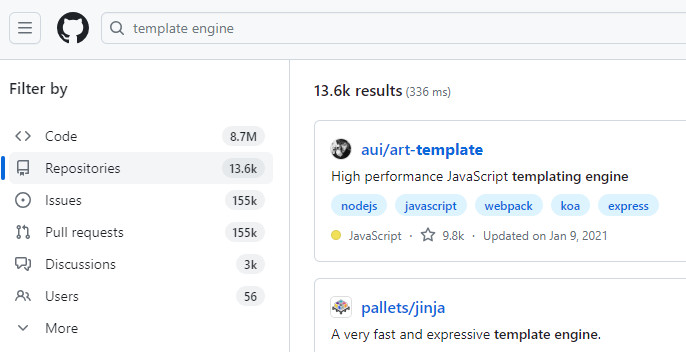
\includegraphics[width=\columnwidth]{Figures/template-engines-2023.png}
\caption{GitHub search for the term `Template Engine' in October 2023}
\label{github}
\end{figure}

Comprehensive comparative information about the many differing implementations can be hard to come by. Software documentation for such tools, where present at all, tends to focus on the use of a single implementation and often reads more like marketing material than a datasheet: emphasising strengths with unverified claims, ignoring weaknesses, and avoiding direct comparison with alternatives.

Template technology is therefore a representative category of software implementation which exhibits the scale, consequences, and lack of easy choices discussed in \autoref{section:motivation summary}. The rest of this chapter will dig deeper into template technology, its characteristics, and the variation between a range of implementations.

\subsection{Concepts and Terminology}

There are several key concepts which inform this research. The intention is to explore these in detail in further sections, but for now, some non-definitive descriptions:

\begin{description}
\item[Template] 

A template is a way of ensuring consistency and reducing re-typing when creating similar documents. Common text and layout are entered just once and then reused to produce many pages or documents. Each template is described in terms of a specific \emph{template language} and designed to be rendered by a compatible \emph{template engine}.

\item[Template Engine] 

A template engine is a software system or component which manages the rendering of \emph{templates}. When an output document is required, the template engine locates an appropriate \emph{template}, loads the data for the desired document into a \emph{page context}, then processes the template by interpreting it according to the \emph{template language} and replacing \emph{placeholder expressions} with appropriate data from the \emph{page context}. 

\item[Template Language] 

A template language specifies how a \emph{template} is expressed. Most template languages consist of a combination of fixed text ready for output (known as `\emph{boilerplate}') and symbolic placeholders. Some template languages use symbolic expressions for everything, including fixed text. Template languages and their placeholder expressions vary widely, but within many template languages it can be useful to consider two types of placeholders: \emph{value expressions} and \emph{control expressions}.

\item[Value Expression] 

A value expression is a sequence of symbols representing the name or location of a data value. When the template is rendered, the value expression will be replaced by a textual version of the data value. If the data value is already textual it will usually just be included in the output. If the data value is numeric or some more complex data type, the way it is rendered will depend on the \emph{template engine} and any options specified in the value expression. The details of the formatting and syntax of such expressions are specified as part of the \emph{template language}.

\item[Control Expression] 

A control expression is not directly replaced by a value in the rendered output, but instead informs the process of rendering the template. Typical control expressions mimic those of conventional programming languages and include, for example: variables, decisions, and loops. Others may have side-effects specific to a particular \emph{template engine} or \emph{template language}.

\item[Page Context] 

A page context is the way that a \emph{template engine} finds data to use when processing \emph{value expressions}. Most \emph{template engines} treat the page context as if it is a simple named data store containing everything needed by the \emph{value expressions} in the \emph{template} currently being processed. However, page context implementations are also available which do not pre-load data before evaluating the \emph{template}, but instead load or calculate data as needed during the processing of the \emph{template}. As each rendered document will potentially be different, a new page context is provided for each document, and the rendering process evaluates the \emph{template} using the specific data from that page context. Depending on the strategy used by the \emph{template engine}, the \emph{template} to use for each document may be determined by examining the page context, or it may be specified externally.

\end{description}

More details of the capabilities and characteristics of template languages and template engines are explored in \autoref{chapter:intermediate}.

\subsection{Templating in the Literature}

There is a substantial body of literature which mentions some form of templating in passing, either philosophically \citep{Bush1945} \citep{Nelson1974} or as a means to achieve a specific end \citep{Caldwell1998} However, while these may contain some information about the selection and use of templating systems, they are not the core of this research. The pool of literature which directly addresses theory and implementation of templates and template languages seems much smaller.

Grouping and categorising is a key way to advance knowledge. \citet{Vegas2009} assert that in science and engineering, knowledge matures as the investigated objects are classified. With the rise in popularity of template approaches, particularly when used to generate web pages, some effort has been put into trying to group template languages and/or template engines into categories to build a body of knowledge and determine unifying constructs; interrelationships; and knowledge gaps \citep{Vegas2009}, with which to reason about capabilities and applicability for different kinds of usage.

\citet{Vosloo2008} set out to survey and classify the landscape of server-side web page generation frameworks. Tellingly they were unable to find other literature at this level of detail:

\begin{displayquote}
This proliferation of discussions and solutions may be construed as an indication that the problem (of finding the right abstractions with which to implement Web-based UI) has not been solved satisfactorily in practice. However, it may also be that the problem merely has a great number of variable parts, and that it needs to be partitioned more usefully. \citep{Vosloo2008}
\end{displayquote}

\citeauthor{Vosloo2008} initially divide the web page technologies they examine according to the three aspects of the popular MVC (Model, View, Controller) pattern. Their research is primarily concerned with what they describe as \enquote{view concerns}. They consider possible taxonomies of page-generation strategies including various forms of templates, eventually presenting the diagram shown in \autoref{diagram:vosloo2008}.

\begin{figure}[ht!]
\centering
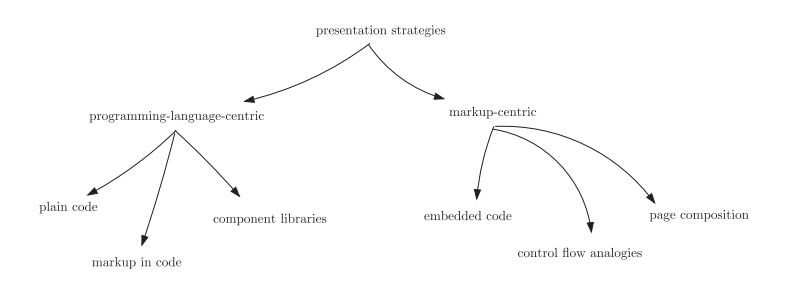
\includegraphics[width=130mm]{Figures/taxonomy.png}
\caption{A Taxonomy of Strategies for View Concerns from \citet{Vosloo2008}}
\label{diagram:vosloo2008}
\end{figure}

The final paragraph of \citeauthor{Vosloo2008}'s \enquote{view concerns} section highlights the usefulness of taxonomy construction in finding under-considered areas:

\begin{displayquote}
For example, none of the 80 frameworks studied relied on a template language with the same basic goal of the page composition variants (Section 5.8), but with a syntax external to the host markup language. ... The absence of such a category in the aforesaid taxonomy could perhaps be the trigger for developing just such a language. \citep{Vosloo2008}
\end{displayquote}

There are, however, two key issues with \citeauthor{Vosloo2008}'s approach. The first is that only server-side web frameworks were considered for the study. While this does not invalidate their results, it does imply that the classification work would need to be re-done if page-generation tools in other technologies, or template techniques for non-web uses were to be included.

Another issue is a more general one with all such taxonomies. As pointed out by \citet{Usman2017} \enquote{most taxonomies are developed in an ad-hoc way}, and \enquote{taxonomies are rarely revisited, revised or extended}. New server-side frameworks and template technologies are continually being produced, and existing ones are continually being revised, updated and re-released. A several-year-old ad-hoc summary is likely to be neither exhaustive nor fully correct and should be considered as a historical source rather than a complete reference. Even with this caveat, though, \citeauthor{Vosloo2008}'s list of 86 server-side web frameworks, most of which have at least some template processing features, begins to show the scale of the problem.

\citet{Laakso2008} also attempt to categorise a selection of web frameworks. As seen in \citet{Vosloo2008}, web frameworks often have template features. \citet{Laakso2008} also have trouble finding prior work on which to base their research:

\begin{displayquote}
To the best of authors' knowledge, very little research has been done about measuring web application frameworks. \citep{Laakso2008}
\end{displayquote}

They do, however, recommend two articles: \citet{Zoio2005} and \citet{Kolesnikov2006}. \citeauthor{Zoio2005} presents a detailed and practical comparison between two frameworks: \emph{JSF}\footnote{\url{https://www.oracle.com/java/technologies/javaserverfaces.html}} and \emph{Tapestry}\footnote{\url{https://tapestry.apache.org/}} through the approach of building the same application twice, once in each of the two competing technologies. \citeauthor{Kolesnikov2006} describes the use of Tapestry in an MSc dissertation.

\citet{Laakso2008} take an experimental approach, as does \citet{Zoio2005}. Both design one or more scenarios, apply them to each of the implementations, and use the results to measure the suitability of different software systems. The comparisons generally concentrate on ease of development and deployment, although there is some mention of rendering performance, which may be analogous to efficiency, and thus affect resource usage. 

Concentrating more specifically on templates, \citet{Parr2004} sets out to 

\begin{displayquote}
formalize the study of template engines, thus, providing a common nomenclature, a means of classifying template generational power, and a way to leverage interesting results from formal language theory. \citep{Parr2004}
\end{displayquote}

\citeauthor{Parr2004}, however, presents the opinion that a template is a pure and separate view and should be "totally divorced from the underlying data computations whose results it will display" (ibid p2) While this is arguably a justifiable position, it does lead to a taxonomy which essentially has two categories: those which enforce such separation, and those which do not. The fully separated category mainly consists of a new template language, \emph{StringTemplate}\footnote{\url{https://www.stringtemplate.org/}}, developed alongside the paper, with almost every other solution relegated to `do not'. \citeauthor{Parr2004} also limits his discussion to template-style solutions written in the Java programming language.

Although \citeauthor{Parr2004}'s \emph{StringTemplate} language has been used for other academic publications \citep{Fritzson2009} \citep{Arnoldus2010} \citep{Hartmann2011} \citep{Arnoldus2012} \citep{Vollebregt2012} and many more, Parr admits that commercial programmers often prefer the features of other, less pure but more powerful, template languages. Implicitly, therefore, there is still a need to categorise these other template languages beyond simply whether or not they enforce separation.

\citet{Arnoldus2010} also addresses the language used in templates, but from a grammatical perspective. The important categorisation distinction in Arnoldus’ work is that of `safety'. Having determined that \enquote{Writing templates, and code generators in general, is a complex and error prone task} (p103), Arnoldus introduces the concept of a `syntax-safe' template, which is incapable of generating grammatically incorrect output. This is particularly important when the output is intended to be machine readable, with a formal grammar, and Arnoldus concentrates on the specific application area of program generation, which exhibits these characteristics. Although Arnoldus does not attempt a categorisation of template languages, he does discuss several key factors (such as the presence of `hedges' (p111), separating placeholder expressions from other text) which are commonly found in those template languages which are more suitable for syntax-safe applications.

\subsection{Discussion}

Templates are the technology of choice for a large proportion of the world's web pages, and thus it seems plausible that the generation of these pages contributes in some part to the large energy and resource usage of the internet and the world wide web.

While there has been some consideration of template engines and template languages in academic literature, the quantity of such papers is dwarfed by the number of software implementations, websites and documentation which have not been through any form of academic peer review process. Template engines and template languages vary widely. Attempts have been made to construct taxonomies in related fields such as web applications, and crowd-sourced information is available from sources such as Wikipedia\footnote{\url{https://en.wikipedia.org/wiki/Comparison_of_web_template_engines}}, but so far, no sign has been found of a detailed and comprehensive comparison and analysis of a wide range of template engine implementations. In the context of this research, so far no taxonomies have been found which include or mention energy consumption, energy-efficiency, or resource usage in general.

It would seem, therefore, that there is an opportunity for research in this field to contribute to knowledge and thereby to potentially assist in improving the overall resource usage of large software systems.

\section{A Feasibility Study}
\label{fs:methodology}
\label{section:fs1}

Even though there are several implementations of template engines mentioned in the literature, there are also many more available. Rather than attempt to gather detailed information about every possible software candidate before starting, the intention was to proceed incrementally, building a collection of data on a growing subset, using preliminary analysis and reflection to inform further research.

Before embarking on a potentially lengthy experimental process, it seemed prudent to attempt to determine whether such research would be likely to provide interesting results. The overall research goal was to help software developers make informed choices to minimise the environmental impact of their work. If measurable differences could be found even between a small selection of software components, then component selection or substitution could be a valid environmental strategy.

With thousands of template engines to choose from, the scope of any initial feasibility study needed to be constrained. Options included limiting the study by popularity, by application domain, by the preferences of specific software developers, by programming language, by template language, by price, or many other factors. Each of these options had theoretical advantages and disadvantages. However, an initial feasibility study needed to be practical and provide results as soon as possible. Following the approach used by \citet{Laakso2008} and \citet{Zoio2005} a study was planned which would select a small number of template components and construct a software test harness to run an identical set of tests on each of the components. There was no attempt to be exhaustive with the selection of components to test.

The aims of the feasibility study were twofold:
\begin{itemize}
    \item To ascertain if this would be a reasonable and useful approach for identifying and comparing template components.
    \item To establish the scale of the variability in features and performance between a sample of available components.
\end{itemize}
Throughout the construction of the study, efforts were made to avoid or constrain `scope creep' \citep{Heinze2014}.

\subsection{Selection of a Programming Language}

To obtain results which could more easily be compared, it was decided to limit the feasibility study to include only template systems in a single programming language. The language \emph{Java} \citep{Oracle2018Java} was chosen for several reasons. Java is generally considered to be one of the most popular programming languages in the world \citep{Tiobe2018}. Java is freely available and runs on a wide range of hardware platforms. Java development tools are also available and familiar to the researcher, reducing both the need for training before commencing the study and the risk of mistakes or misunderstandings.

\subsection{Selection of Template Engines}

The next stage was to select an initial set of template engines for the feasibility study.

\begin{table}
\centering
\begin{tabular}{c|p{3in}}
  \toprule
  \textbf{Template Engine} & \textbf{Reasons for Selection} \\
  \midrule

  \makecell{
    \emph{StringTemplate}\tablefootnote{\url{https://www.stringtemplate.org/}} } & 
  Cited several times in academic literature \\
  \midrule

  \makecell{
    \emph{Velocity}\tablefootnote{\url{https://velocity.apache.org/}} \\
    \emph{FreeMarker}\tablefootnote{\url{https://freemarker.apache.org/index.html}} } & 
  Popular in lists of Java template engines on the web \\
  \midrule

  \makecell{\emph{Mustache}\tablefootnote{\url{https://mustache.github.io/}} } & 
  Probably the most widely implemented style of template engine, with implementations in at least 45 Languages \\
  \midrule

  \makecell{
    \emph{Jangod}\tablefootnote{\url{https://code.google.com/archive/p/hapax/}} } & 
  An alternative implementation with syntax somewhat similar to \emph{Mustache} \\
  \midrule

  \makecell{
    \emph{Hapax}\tablefootnote{\url{https://code.google.com/archive/p/hapax/}}  } & 
  A template engine implementation with syntax partially similar to Mustache but with internal differences \\
  \midrule

  \makecell{
    \emph{Casper}\tablefootnote{\url{https://code.google.com/archive/p/casper/}} } & 
  Processes placeholders using an embedded JavaScript interpreter \\
  \midrule

  \makecell{
    \emph{JMTE}\tablefootnote{\url{https://github.com/HubSpot/jmte}} } & 
  Pre-compiles templates into Java class files for execution \\
  \midrule

  \makecell{
    \emph{Stringtree}\tablefootnote{\url{https://github.com/efficacy/stringtree}} \\ \emph{Solomon}\tablefootnote{\url{https://bitbucket.org/efficacy-misc/emo/src/master/src/main/java/org/stringtree/solomon/}} } &
  Implementations resulting from previous personal research in this area \\

\bottomrule
\end{tabular}
\caption{Reasons for Selection of Template Engines\label{table:software-reasons}}
\end{table}

\subsection{Construction of a Feasibility study}

Keeping the feasibility study aims in mind, the following eight simplified \enquote{real world} evaluation scenarios were constructed:

\begin{description}
\item[Scenario S0: No substitutions (`control' case)] \hfill

The job of a template engine is to read and combine a template with some variable data by replacing placeholders. However, not all template documents contain placeholders. Some are just documents to be served unchanged. The processing within the template engine will likely add some overhead. This scenario gives some indication of the processing overhead in each implementation.

\item[Scenario S1: A single textual substitution] \hfill

The simplest active case for a template engine is the identification of a placeholder and its replacement with a single constant textual value. The purpose of this scenario is to evaluate the performance of this common activity.

\item[Scenario S2: A collection of textual values] \hfill

A step up from a single value is the substitution of a collection (such as an array, a list, or some other iterable object) of textual values. This scenario requires the template engine to determine in some way that the value to be substituted is a collection, and to make some attempt at rendering the contents in order.

\item[Scenario S3: A collection separated by commas] \hfill

It is usual in English when presenting a list to separate the items with commas. Given the list (\emph{ham} \emph{eggs} \emph{chips}) it might be typical to present it as \texttt{ham, eggs, chips} (or even \texttt{ham, eggs, and chips}, but that is less common in dynamically generated documents, and beyond the scope of this feasibility study). This scenario is an interesting challenge for a template engine, which is why it is a separate test from simply rendering the contents of a collection. Some template engines make it difficult to avoid placing an excess comma after the final item, for example.

\item[Scenario S4: Include another template] \hfill

Structural decomposition (colloquially known as \emph{divide and conquer}) is a key practice of software engineering, and also applies to the design and construction of documents such as web pages from component parts. For this to work, a template system must be able to include within its output the result of processing another template. This scenario evaluates the effectiveness of a template engine at constructing compound documents.

\item[Scenario S5 and S6: Show a value if a boolean value is \emph{true} or \emph{false}] \hfill

Conditional execution is another key aspect of software. In the case of template processing it is a common requirement to show a true/false value from the data as text. From a single letter or a glyph such as an emoji or checkmark (\checkmark) to a swathe of boilerplate or a whole extra template, the process is the same. If the value is true, show the specified text. Some template languages make a big issue of the difference between showing some text if true, but nothing at all if false, and showing alternative text such as \checkmark for true and $\times$ for false. These scenarios evaluate the effectiveness of a template system at converting boolean values.

\item[Scenario S7: Call some code] \hfill

Although \citeauthor{Parr2004} considers this a \enquote{violation} of the principle of separation of logic from display, many template systems support the execution of arbitrary code during the rendering of templates. Techniques for achieving this vary widely, but with the Java ecosystem there is a standard way of invoking code from other contexts: the \emph{JavaBeans} API \citep{Oracle2018JavaBean}. Use of this API allows systems such as template engines to execute an object method by treating it as accessing a data field. Typical uses for this facility in a template is to include data which is expensive to pre-calculate or may not be known in advance. This scenario evaluates the effectiveness of a template system at using the \emph{JavaBeans} API.

\end{description}

\subsection{Implementation of a Feasibility Study}

One of the characteristics which separates template systems is the variation in their template languages. An implication of this is that templates cannot usually be re-used to evaluate different template engines. These distinctions, and some approaches to minimising their impact, are explored in more detail in \autoref{chapter:intermediate}. Likewise, template engines provide a variety of software interfaces.

For best compatibility of test results tests should be as similar as possible, yet the nature of the different template engines requires many differences in implementation. To resolve these tensions, an architecture was chosen which used the strategy pattern \citep{Gamma1994} to enable isolation of specific differences between the code for the various template engines.

\begin{figure}[ht!]
\centering
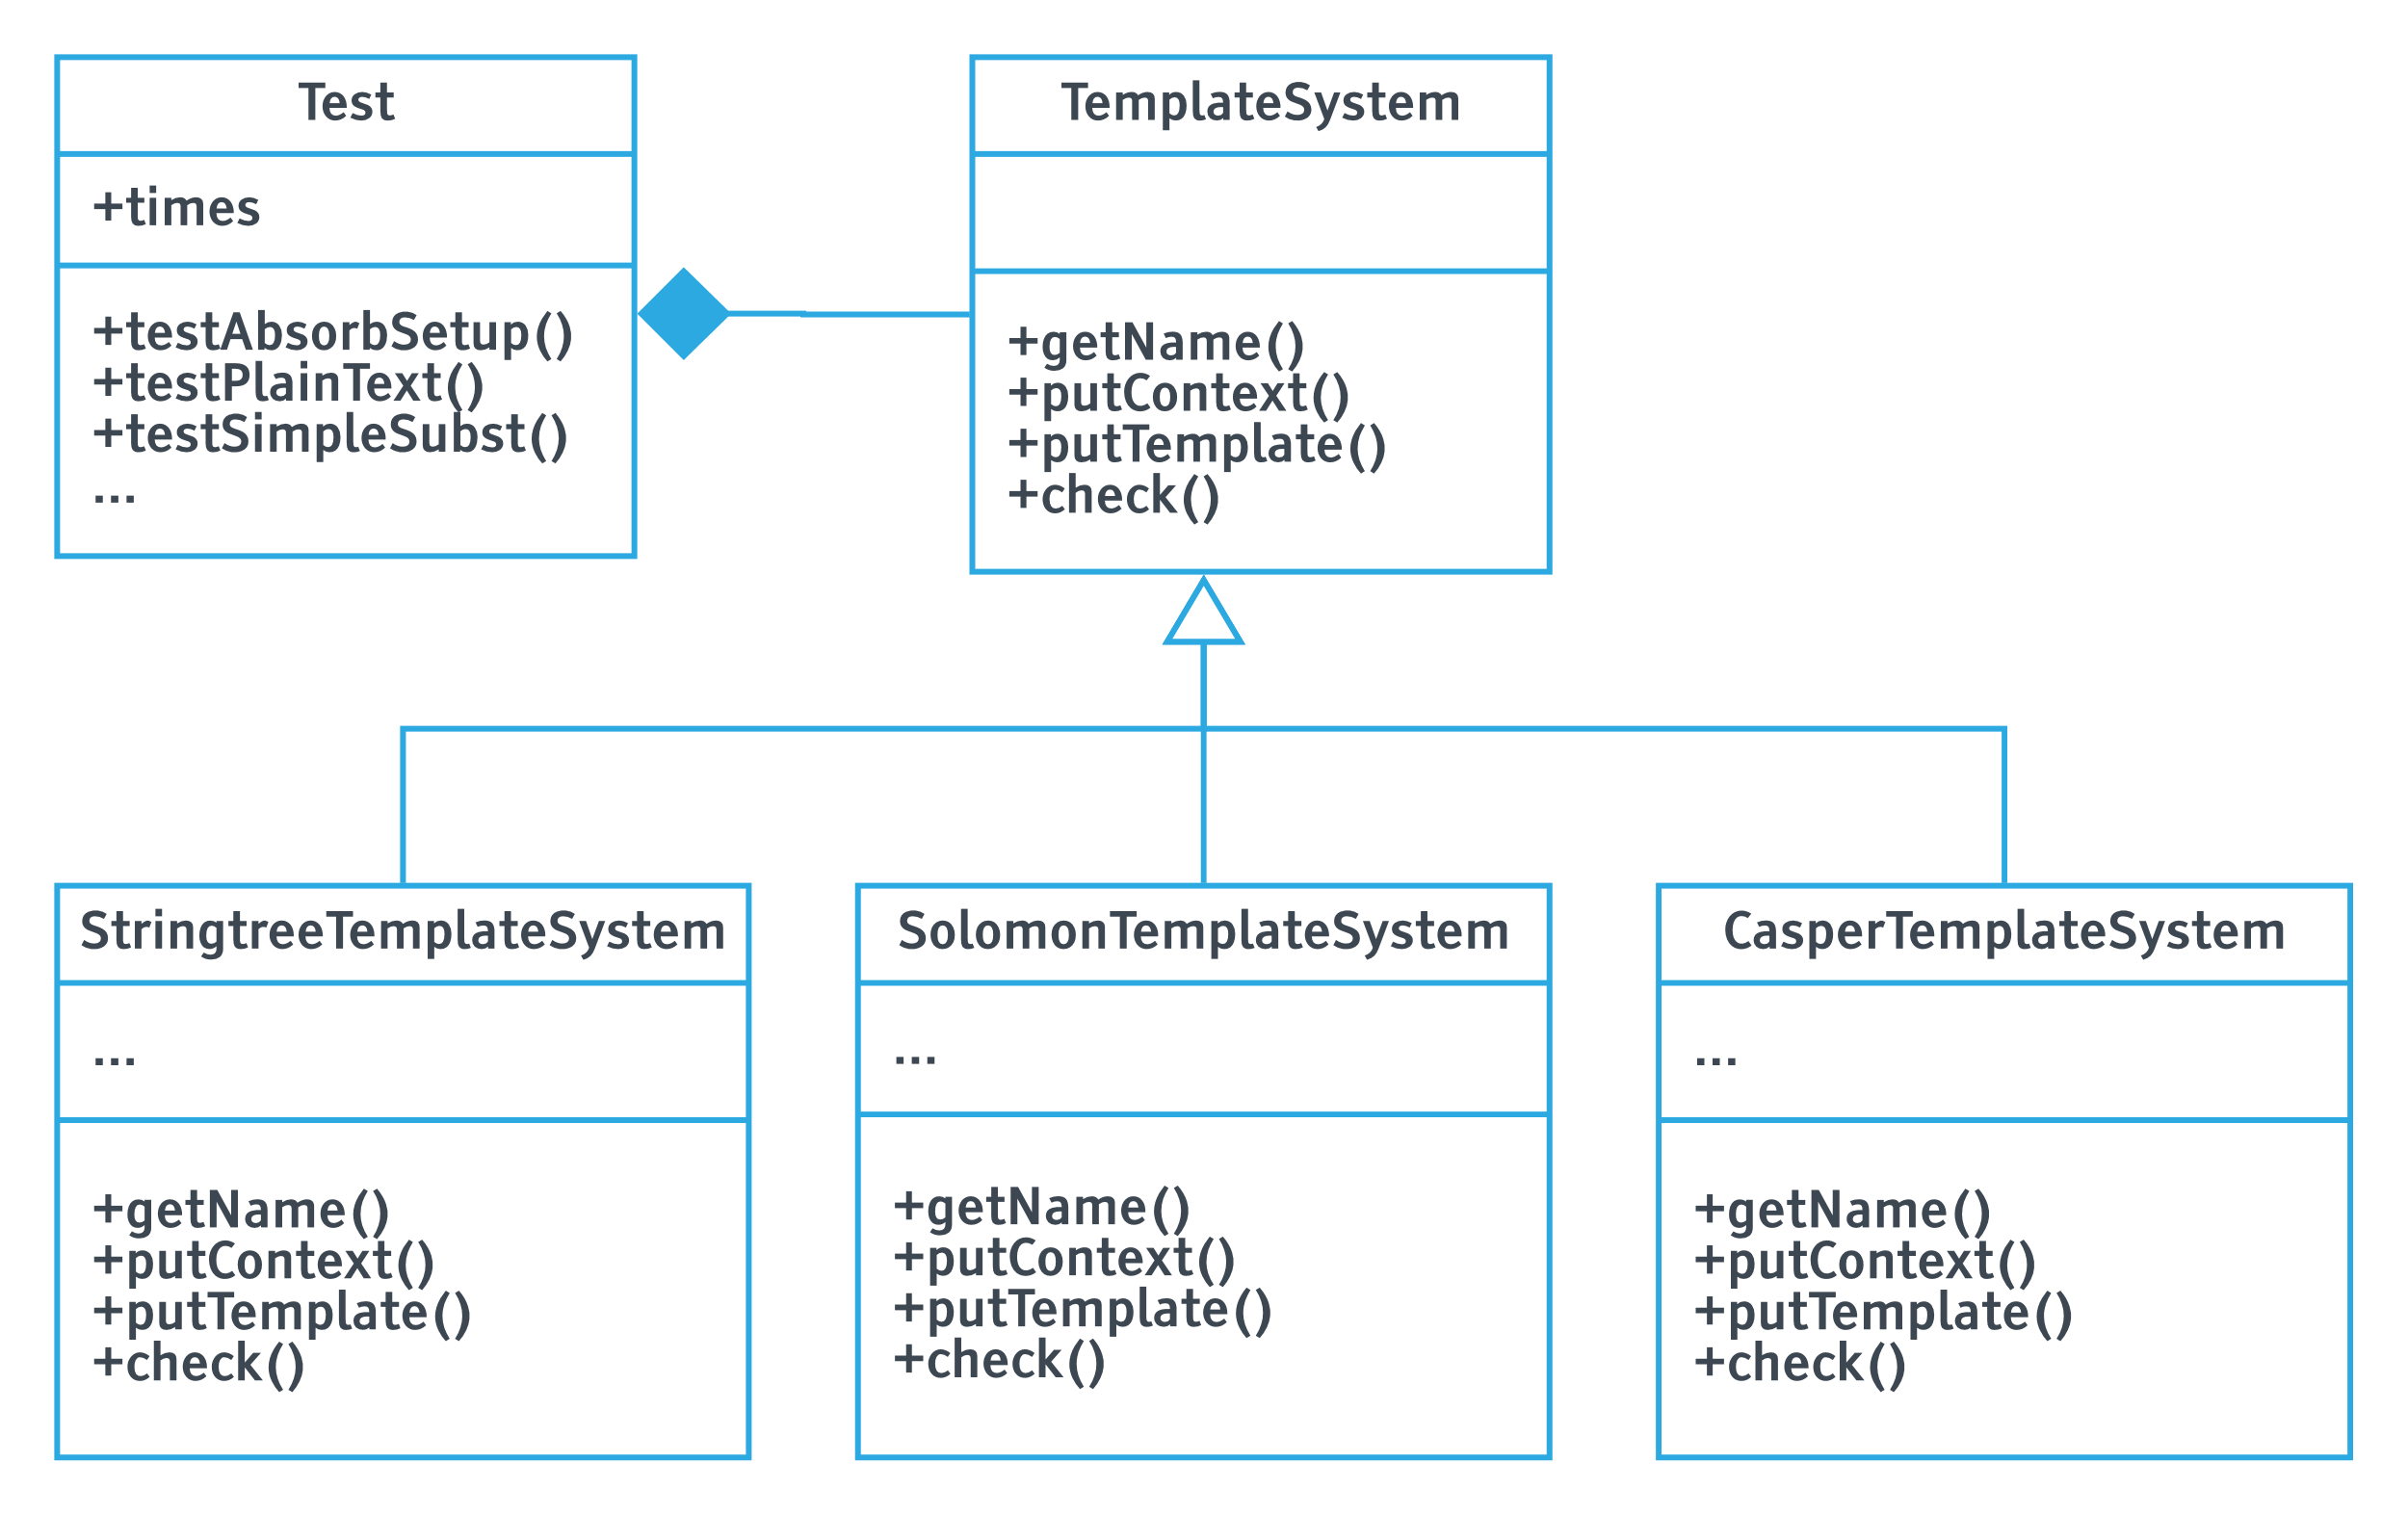
\includegraphics[width=130mm]{Figures/classes.png}
\caption{Class diagram showing use of strategy pattern}
\label{fs:figure:strategy}
\end{figure}

As each concrete strategy class was coded and tested, it was integrated with a test harness written using the JUnit test library\footnote{\url{https://junit.org/}}. When all implementations were complete, code was added to compare generated output with expected output from each test for each test harness, and to time multiple runs of each such test. Tests were timed using the Java \texttt{System.currentTimeMillis()} method, which uses the system `wall clock' rather than attempting to measure only time used by specific processes or threads.

The code for the test harness underwent several changes as the template implementations were added. Most commonly this was due to differing assumptions between implementations. For example, many template engines expect to fetch templates from a local file system but some prefer other means, so the abstract definition of the strategy implementations had to change to support a wider variety of such sources. As much as possible, however, such changes were kept in the common part of the code rather than being duplicated in template-specific classes.

Despite copious reading of documentation, source code and web articles, it was not possible to coerce all template engines to generate fully correct output for all test scenarios. Such failures are noted in the results but it was decided not to exclude these test scenarios from the timed tests.

As testing progressed it became apparent that performance of the differing template engines varied widely, so the timed part of the experiment was tuned to give all the template engines a chance to complete in a reasonable time. Eventually a value of 10,000 repetitions was settled on as an effective number. This gave largely repeatable results for each template engine.

\section{Feasibility Study Results}
\label{fs:results}

The success of the test scenarios is given in \autoref{fs:table:features}, and the timings for 10,000 runs of each scenario are given in \autoref{fs:table:times}.

\begin{table}[ht!]
\fontsize{9}{11}\selectfont
  \begin{center}
    \begin{tabular}{rllllllll}
      & {\rotatebox{90}{{\textbf{S0 No Subst}}}} 
      & {\rotatebox{90}{{\textbf{S1 Single Text}}}} 
      & {\rotatebox{90}{{\textbf{S2 Collection}}}}
      & {\rotatebox{90}{{\textbf{S3 Separated}}}}
      & {\rotatebox{90}{{\textbf{S4 Include}}}}
      & {\rotatebox{90}{{\textbf{S5 Bool True}}}}
      & {\rotatebox{90}{{\textbf{S6 Bool False}}}}
      & {\rotatebox{90}{{\textbf{S7 Call Code}}}}\\
      \toprule
      \textbf{Solomon} & \checkmark & \checkmark & \checkmark & \checkmark & \checkmark & \checkmark & \checkmark & \checkmark\\
      \textbf{Stringtree} & \checkmark & \checkmark & \checkmark & \checkmark & \checkmark & \checkmark & \checkmark & \checkmark\\
      \textbf{JMTE} & \checkmark & \checkmark & \checkmark & \checkmark &  & \checkmark & \checkmark & \checkmark\\
      \textbf{Mustache} & \checkmark & \checkmark &  &  & \checkmark & \checkmark & \checkmark & \checkmark\\
      \textbf{Stringtemplate} & \checkmark & \checkmark & \checkmark & \checkmark & \checkmark & \checkmark & \checkmark & \\
      \textbf{FreeMarker} & \checkmark & \checkmark & \checkmark & \checkmark & \checkmark & \checkmark & \checkmark & \checkmark\\
      \textbf{Velocity} & \checkmark & \checkmark & \checkmark &  & \checkmark & \checkmark & \checkmark & \checkmark\\
      \textbf{Hapax} & \checkmark & \checkmark & \checkmark &  &  &  &  & \\
      \textbf{Casper} & \checkmark & \checkmark & \checkmark & \checkmark & \checkmark & \checkmark & \checkmark & \checkmark\\
      \textbf{Jangod} & \checkmark & \checkmark & \checkmark &  & \ & \checkmark & \checkmark & \\
    \end{tabular}
  \end{center}
\caption{Test successes by template engine and scenario}
\label{fs:table:features}
\end{table}


\begin{table}[ht!]
\resizebox{\textwidth}{!}{
    \begin{tabular}{rrrrrrrrrSS}
      & {\rotatebox{90}{{\textbf{S0 No Subst}}}} 
      & {\rotatebox{90}{{\textbf{S1 Single Text}}}} 
      & {\rotatebox{90}{{\textbf{S2 Collection}}}}
      & {\rotatebox{90}{{\textbf{S3 Separated}}}}
      & {\rotatebox{90}{{\textbf{S4 Include}}}}
      & {\rotatebox{90}{{\textbf{S5 Bool True}}}}
      & {\rotatebox{90}{{\textbf{S6 Bool False}}}}
      & {\rotatebox{90}{{\textbf{S7 Call Code}}}}
      & {\rotatebox{90}{\textbf{\emph{Mean}}}}
      & {\rotatebox{90}{\textbf{\emph{SD}}}}
      \\
      \toprule
      \textbf{Solomon} & 4 & 4 & 17 & 2 & 8 & 7 & 2 & 20 & \textbf{8} & \textbf{6.87}\\
      \textbf{Stringtree} & 133 & 62 & 119 & 77 & 109 & 83 & 56 & 53 & \textbf{86.5} & \textbf{30.43}\\
      \textbf{JMTE} & 9 & 13 & 46 & 3 & \emph{(30)} & 10 & 9 & 11 & \textbf{17.4} & \textbf{14.30}\\
      \textbf{Mustache} & 396 & 275 & \emph{(631)} & \emph{(461)} & 453 & 361 & 377 & 396 & \textbf{418.8} & \textbf{103.36}\\
      \textbf{Stringtemplate} & 239 & 243 & 322 & 150 & 350 & 158 & 92 & \emph{(40)} & \textbf{196.6} & \textbf{108.42}\\
      \textbf{FreeMarker} & 25 & 17 & 29 & 34 & 40 & 22 & 37 & 28 & \textbf{29} & \textbf{7.75}\\
      \textbf{Velocity} & 252 & 168 & 282 & \emph{(250)} & 205 & 178 & 124 & 114 & \textbf{196.6} & \textbf{61.58}\\
      \textbf{Hapax} & 64 & 79 & 124 & \emph{(58)} & \emph{(117)} & \emph{(43)} & \emph{(49)} & \emph{(55)} & \textbf{73.6} & \textbf{30.88}\\
      \textbf{Casper} & 19311 & 15878 & 23783 & 18226 & 27997 & 21292 & 21572 & 21048 & \textbf{21138.3} & \textbf{3,659.57}\\
      \textbf{Jangod} & 145 & 158 & 187 & \emph{(270)} & \emph{(126)} & 127 & 117 & \emph{(313)} & \textbf{180.5} & \textbf{72.94}\\
      \hline
      \textbf{Range} & \textbf{19307} & \textbf{15874} & \textbf{23766} & \textbf{18224} & \textbf{27989} & \textbf{21285} & \textbf{21570} & \textbf{21037}   &  & \\
      \textbf{Relative Diff.} & \textbf{4827.75} & \textbf{3969.50} & \textbf{1399.00} & \textbf{9113.00} & \textbf{3499.63} & \textbf{3041.71} & \textbf{10786.00} & \textbf{1913.45}   &  & \\
      \textbf{SD} & \textbf{6063.46} & \textbf{4986.19} & \textbf{7461.39} & \textbf{5719.58} & \textbf{8804.06} & \textbf{6699.23} & \textbf{6792.19} & \textbf{6621.10}   &  & \\
      \textbf{SD (exc. \emph{Casper})} & \textbf{133.51} & \textbf{101.89} & \textbf{195.61} & \textbf{154.78} & \textbf{151.65} & \textbf{113.90} & \textbf{113.96} & \textbf{140.82}   &  & \\
    \end{tabular}
}
\caption{Time (ms) taken for 10,000 runs by template engine and scenario}
\label{fs:table:times}
\end{table}

\begin{figure}[ht]
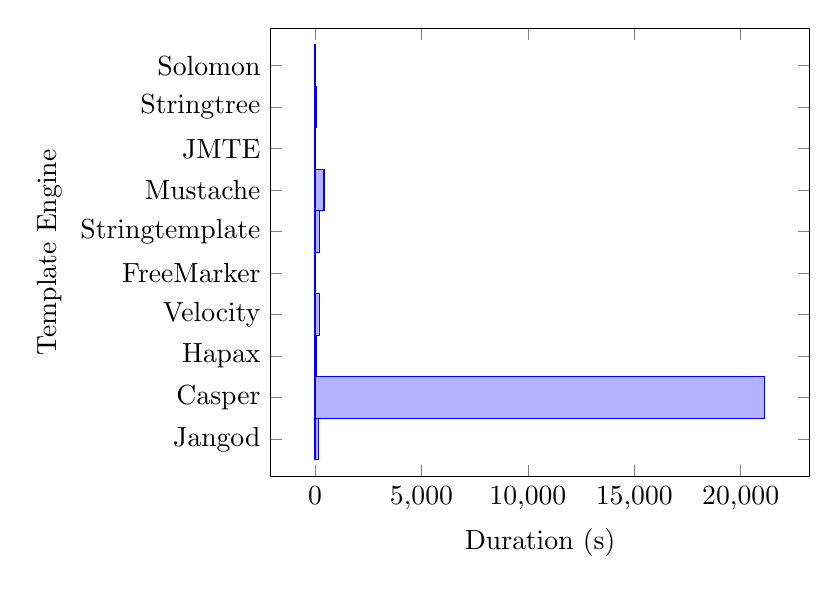
\begin{tikzpicture}
\begin{axis}[
    scaled ticks=false,
    % xmode=log,
    % ticks with fixed point,
    % scaled ticks=false,
    xbar stacked,
	bar width=15pt,
	% nodes near coords,
    ytick=data,
    legend style={at={(0.5,-0.20)},
      anchor=north,legend columns=-1},
    ylabel={Template Engine},
    xlabel={Duration (s)},
    symbolic y coords={
        Jangod, Casper, Hapax, Velocity, FreeMarker,
        Stringtemplate, Mustache, JMTE, Stringtree, Solomon
    },
    ]
\addplot+[xbar] plot coordinates {
  (180.5,Jangod) (21138.3,Casper) (73.6,Hapax) (196.6,Velocity) (29,FreeMarker)
  (196.6,Stringtemplate) (418.8,Mustache) (17.4,JMTE) (86.5,Stringtree) (8,Solomon)
};
\end{axis}
\end{tikzpicture}
\caption{Mean test duration by template engine}
\label{fs:graph:duration}
\end{figure}

\begin{figure}[ht]
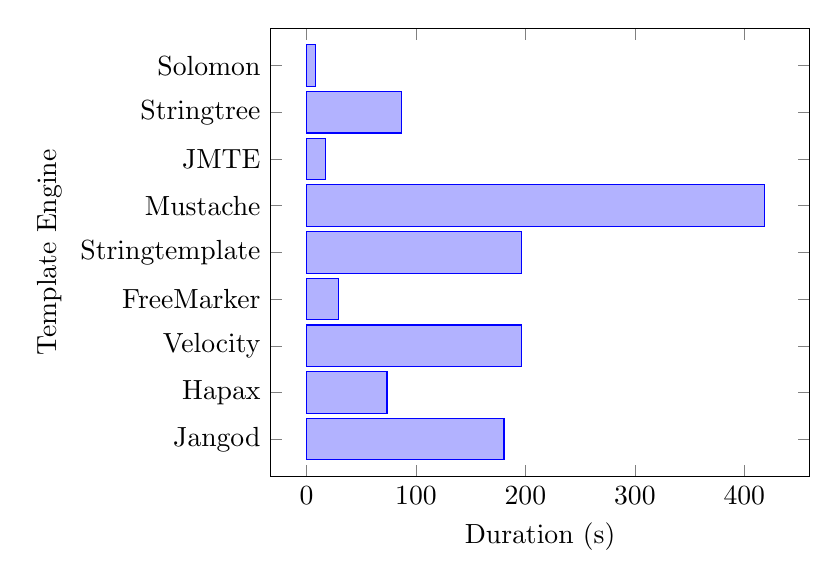
\begin{tikzpicture}
\begin{axis}[
    scaled ticks=false,
    % xmode=log,
    % ticks with fixed point,
    % scaled ticks=false,
    xbar stacked,
	bar width=15pt,
	% nodes near coords,
    ytick=data,
    legend style={at={(0.5,-0.20)},
      anchor=north,legend columns=-1},
    ylabel={Template Engine},
    xlabel={Duration (s)},
    symbolic y coords={
        Jangod, Hapax, Velocity, FreeMarker,
        Stringtemplate, Mustache, JMTE, Stringtree, Solomon
    },
    ]
\addplot+[xbar] plot coordinates {
  (180.5,Jangod) (73.6,Hapax) (196.6,Velocity) (29,FreeMarker)
  (196.6,Stringtemplate) (418.8,Mustache) (17.4,JMTE) (86.5,Stringtree) (8,Solomon)
};
\end{axis}
\end{tikzpicture}
\caption{Mean test duration excluding Casper}
\label{fs:graph:duration-excluding}
\end{figure}

\section{Feasibility Study Analysis}
\label{fs1:analysis}

It is reassuring that all the template systems in the study were capable of processing both plain text (S0) and simple substitution (S1) cases. However, these were the only scenarios which everything passed. For all the other test scenarios there was at least one template engine which could not manage it. There were only four template engines in the sample which correctly rendered every scenario: \emph{Solomon}, \emph{Stringtree}, \emph{Freemarker}, and \emph{Casper}. Given that these scenarios were chosen as representative of common situations in professional software development, it is surprising that there was so much variability in features. The documentation for all the implementations makes some kind of claim of being `powerful', `flexible' or `suitable for a wide range of projects'. 

Consider, for example, the \emph{Hapax} template system which failed five of the eight tests. Its documentation states:

\begin{displayquote}
Hapax is a simple but powerful text templating library for Java. Hapax is suitable for constructing text output from Java code. The syntax is similar to Google's ctemplate library, and emphasizes the separation of logic from presentation. Hapax was designed to be easy to use and have minimal dependencies. Hapax does not depend on any existing web framework, and is suitable for use in servlets, scripting languages (Scala, Groovy, etc), and server-side applications.
\end{displayquote}

Nowhere in this does it mention any limitations, making comparing implementations on documentation alone a tricky proposition. Attempts have been made to compile comparative lists of such software by features \citep{Wikipedia2018} but interpretation of the exact meaning of each feature can be loose, and there would potentially be great benefit in defining a comprehensive set of such benchmark scenarios which could be used to compare and evaluate even software which is not found in such lists. The production of such benchmark scenarios would be difficult, however, because of the wide differences between template languages. There is currently no single `meta language' in which scenarios can be expressed for multiple template engines. This problem is explored further in \autoref{chapter:intermediate}.

In many cases the limitations of the template engines seem closely tied to the choice of template language. The minimalist language common to many \emph{Mustache} implementations, for example, deliberately avoids constructs such as loops, in favour of performing such logic in application code before invoking the template engine. While this can be a workable strategy, and satisfies \citeauthor{Parr2004}'s (\citeyear{Parr2004}) desire for separation of concerns between view and model, it also has some potential drawbacks. Preparing values requires extra processing in the application code, which partially disguises the processing cost of generating pages compared to more competent template engines. It also requires that every possible configuration of data for the page is pre-calculated, including `expanding' collections. While expanding lists of textual or numeric values is relatively simple, this approach becomes much more complex in the relatively common case where each entry in the list needs to be processed using a secondary template in order to generate the desired result. This approach also denies the template engine any possibility of automatically re-using intermediate values or using `lazy evaluation' strategies to avoid unused calculations, for example when Boolean conditions remove the need for a value to be rendered. Such choices have considerably more impact when the same application code is used to evaluate a wide variety of templates, each with different data requirements. In common with many software development habits, which prioritise development effort over execution time, it can be easier for developers to produce general-purpose code which pre-calculates everything required by every possible template, even though many of those values will not be required for any given rendered page. This can add extra, unneeded, processing cost to every page.

There is also an anomaly in the timings. In table 3.2, it appears that several of the template engines take longer to process a plain text file than a simple substitution. While this is possible, it seems somewhat unlikely, so the experiment was temporarily adjusted to run the tests in a different order. Whichever test runs first seems to take longer. The current hypothesis is that this is an artefact of some kind of “warm up” behaviour, either in the template engine code or in the Java language and runtime. This implies that the data in table 3.2 should not be used to compare performance across scenarios for any given template engine, but the the experiment remains useful for comparing the range of performance between template engines.

The software `test bench' for these measurements was constructed using the strategy pattern (as shown in \autoref{fs:figure:strategy}) with all the template engine libraries loaded into memory at the same time. This made running the experiments much simpler, as they could be performed by a simple loop through a collection of \emph{TemplateSystem} objects with no need to stop or start the code, or to add and remove external code blocks. However, this approach also required some careful coding to deal with potential clashes and incompatibilities between the separate template libraries and their transitive dependencies. The version of Java used for these experiments did not provide any form of separation between libraries beyond class and package names. Any problems with any of the template engine implementations (such as a syntax error in a template specification) which caused the template engine to `crash' or raise an exception, would abort the whole test run. It is not clear whether there was any more subtle interference between the separate libraries which may have affected the results.

The approach of treating this code as a `throw away' experiment and writing only the minimum code necessary to perform the experiments had an impact on the usability of the software. Result values were simply printed out as soon as they were calculated, without performing any analysis or data formatting. This required manual copying into analysis software to determine derived results such as the mean duration. Configuration parameters such as the collection of template engines to be tested and the number of times to invoke them were hard-coded into the software, which meant that any change required editing and re-compliation of the experiment code.

Finally, it is important to note that this feasibility study only measured two things: the ability to correctly render some specific scenarios, and the time taken to perform them. While some \emph{guesses} may be made about what that might mean for overall energy usage, this study does not say anything definitive about the energy usage of the different template engines.

Further research is needed to address the above issues. Methods of measuring the energy usage of software are explored in \autoref{chapter:testrig} .Improvements to the construction and operation of the test framework and more detailed  comparison of component performance are discussed in \autoref{section:fs2}.

\subsection{Analysis of Individual Template Engines}

It is clear from \autoref{fs:table:times} that performance of different template engines varies widely. Examining the code of the outliers (\emph{Solomon}, the fastest, and \emph{Casper}, the slowest) shows some interesting features. Casper has obviously been designed to be as flexible as possible, going so far as to start a complete JavaScript interpreter for every page generated, and discarding it when the page is completed. This imposes a relatively huge burden on generating regular web pages but does potentially provide some facilities unavailable in most other systems. It is important to note that this feasibility study was designed based on common web page scenarios, and thus does not include any cases where Casper would be the only applicable solution. Solomon, on the other hand has been coded solely for speed. It uses a relatively non-standard template language, optimised for simple and fast processing rather than easy readability and the internal design minimises buffering and data copying. One other template engine in this study (\emph{Stringtree}) uses a similar template language to Solomon but does not achieve the same performance benefits. When Stringtree was coded, performance was not the primary goal.

\emph{Casper} takes so long to perform the experiments that it makes \autoref{fs:graph:duration} unusable for comparing the performance of the other template engines. By removing Casper from the results (see \autoref{fs:graph:duration-excluding}) a more nuanced view of their relative performance can be seen. In this figure, template engine performance can be seen to cluster into a few groups. \emph{Mustache} is in a group of its own, at over 400s, taking roughly twice the time as the engines in the next group. The next group contains three template engines: \emph{Stringtemplate}, \emph{Velocity}, and \emph{Jangod} all of which take around 200s. A third group includes \emph{Hapax} and \emph{Stringtree} which both take a bit less than 100s to complete the run. The final, fastest, group includes \emph{Solomon}, \emph{JMTE}, and \emph{Freemarker}, all taking 30 seconds or less.

If the above experiments were used to select a template engine for a project based on performance, then the three template engines in the fastest group would form the short-list. Selecting between these three would then depend on further factors. \emph{Solomon} is clearly the fastest, and it is able to correctly perform all the scenarios, so is the obvious choice. However, Solomon uses a slightly unusual template language which could hinder adoption. JMTE is the second fastest, but could not correctly perform all the scenarios. In development situations where the missing features are not important, however, then JMTE could be a good compromise. \emph{Freemarker}, although it is up to 18 times slower than Solomon for some cases, was the only popular template engine to correctly perform all the scenarios. \emph{FreeMarker} also has the advantage of a well-documented template language and wider adoption than the other two, so would also make a good choice for a more conservative development team. Based on their performance it would seem a poor choice to select any of the others.

\section{Feasibility Study Discussion}
\label{fs:discussion}

A key finding to arise from the feasibility study is the surprising variety in capabilities and performance between purportedly similar software libraries. For some common operations in this study there was over 10,000 times difference between the best and the worst performers. Even averaged across the range of different operations, the difference in time taken to perform the same task is still over 2,500 times between the best and worst performing libraries.

Such stark contrast is nowhere to be found in the documentation, however, which makes selecting a template engine for use in a software project a difficult task. All the components evaluated in this study are free software, so the traditional approach of minimising the purchase cost does not apply. All the components are available with licences which permit inclusion in commercial software, so considering licence terms is also no use in selecting between them. Despite their free availability, and with no direct financial incentive to increase `sales', they often provide documentation which reads like optimistic and unsubstantiated advertising copy. Such documentation as is provided tends to concentrate on listing and describing specific available features, covering everything else with blanket subjective statements such as `fast', `powerful' or `flexible'. This paucity of information makes it hard for developers to make informed choices.

The fact that one template engine, \emph{Solomon}, was able to correctly perform all the scenarios in a much faster time than any of the others when they are all written in the same programming language and running on the same platform, shows that the choices made in the design and programming of the different template engines in this study have had a huge impact on the performance and capabilities of these supposedly equivalent components. In this specific case, one reason could be that \emph{Solomon} was written to minimise multiple handling of template characters. Whenever possible, input characters are passed directly to the output document without buffering. The characteristics of the \emph{Solomon} template language (discussed in more detail in \autoref{section:comp:languages}) help reduce the need for buffering.

\section{Feasibility Study Conclusions}
\label{fs:conclusions}

In conclusion, preliminary results show that there is a surprisingly wide range of difference in capabilities and performance between superficially similar solutions to a specific class of problem. The study provides data which was not clear from the on-line documentation for the components being considered. This in turn suggests that a change in software development behaviour, both when writing software and when selecting components or libraries, could potentially make a noticeable difference in overall energy and resource usage of large software systems such as the world wide web. Further research is required to explore and quantify this impact.

In particular, the following specific conclusions will be taken forward from this feasibility study:

\begin{itemize}
\item The differences between this sample of components are large enough to be worth proceeding with the research.
\item Choices made during design and development of software, and when selecting components, can have a large impact on the performance of the final product.
\item The methodology of constructing a range of representative scenarios and using them to compare the different components is fundamentally sound, however, improvements are needed to the implementation of the tests
\item The template languages used by the different template engines vary widely enough that further research is needed on ways to simplify the creation of equivalent templates for a range of template engines.
\item Further research is needed to determine what impact this wide variety in performance might have on energy usage.
\end{itemize}

\section{An Improved Performance Study}
\label{section:fs2}

The following sections address the shortcomings of the feasibility study to enable a deeper exploration of the performance characteristics of template engine components.  The development of an improved framework for the evaluation of components, and the results from using it for a wider range of performance comparisons is discussed in \autoref{section:comp:framework}.

\subsection{Recap of Problems With The Feasibility Study}
\label{section:comp:recap}

The feasibility study was conducted to gain an overview of the scale of the differences between a selection of components. While the results were clear, the individual performance measurements were neither rigorous nor comprehensive. In particular, the following issues were discovered:

\begin{itemize}
    \item \textbf{Problem 1} All the template engines were loaded into memory at the same time, which could cause influence between different components.
    \item \textbf{Problem 2} Clashes, both between class and package names of components and where components required different versions of the same library.
    \item \textbf{Problem 3} Configurations were all hard-coded, requiring editing and re-compilation of the code   \item \textbf{Problem 4} An anomaly in the timings where whichever scenario was run first took extra time.
    \item \textbf{Problem 5} Scenarios were always run the same number of times, and therefore showing only how the components compare at that load.
    \item \textbf{Problem 6} Results output was simplistic and difficult to process.
\end{itemize}

\subsection{Changes to the Component Landscape}

All of the template engine components evaluated as part of the feasibility study were open source and free of charge and were chosen to be broadly representative of the available software at the time. In the period between the feasibility study and the later measurements of the components, however, the landscape of software in this niche had changed and developed. This is a natural process in open source software \citep{Sonatype2023} \citep{Xie2009}. While the template engines evaluated in the feasibility study were all still available, many had not been updated or were no longer in popular use. Several other template engines had appeared or increased in popularity in the intervening time. More research was needed to determine an appropriate set of template engines to evaluate in more detail.

\section{Selecting Template Engines to Compare}
\label{section:comp:selecting}

For this stage of the research a more systematic approach was needed. This comprised the following initial steps to build a list of candidate template engines:

\begin{enumerate}
    \itemsep -0.5\parsep
    \item Limit the search to the \emph{GitHub}\footnote{\url{https://github.com/}} code repository
    \item Perform a search for the term `template engine'.
    \item Limit the results to code in the Java language.
    \item Ignore repositories which are not textual template engines in their own right such as adaptors, plugins, examples, game engine templates etc.
    \item Ignore special-purpose template engines with specific output formats such as PDF, DOCX, and SQL.
    \item Ignore template engines which are obviously based on the `Template Engine Kata' from \citet{Koskela2007}.
    \item Ignore template engines which are `forks' of other template engines in the list
    \item Ignore template engines with documentation in languages other than English.
\end{enumerate}

This process resulted in a list of 132 template engines. The full list with names and GitHub URLs can be found in \autoref{appendix:engines}. Note that, as mentioned above, the open source software landscape is continually changing, so following the same process at a later date would produce a different, and probably larger, set of results.

\subsection{Sources of Information}

Even having eliminated the obvious cases where template engines appeared to have been created purely as a learning aid, there were still many in the list which were either incomplete, unusable, or would be unlikely to be used by anyone other than the original developer. To get perspective on which template engines to consider further, some gauge of popularity was needed.

Unfortunately, there is no single resource which indicates the popularity of such software components. Commercial products do not usually reveal their choice of components. Some code repositories provide indications of the number of times a particular component has been downloaded, or how many times it is used by other projects in the same repository. While such statistics can give clues as to the popularity of components, they are not reliable. For example, download counts are easily skewed if some organisation has a policy of re-downloading every component for every build, which may happen many times per day. Statistics on the usage of components by other components are arguably more useful, but are limited to dependencies that the repository is aware of, and do not include code which is not stored in a public component repository.

On the wider internet, there are a range of personal and collaborative websites containing recommendations and comparisons. These websites can provide an indication of popularity. Individually, each such website is of limited use. The information provided may not be objective and has probably never been reviewed. The site may be out of date, presenting information on obsolete versions of components. The authors may have misunderstood the capabilities of individual components, or be unaware of the existence of some, or lack the skills or experience to fully evaluate the options. In some cases the information may be deliberately or accidentally biased.

When a range of such resources are considered as a whole, however, they can provide a kind of `zeitgeist', but there are still potential problems. While outright collusion is less likely when a broad enough group of websites is included, there is still the possibility of an `echo chamber' effect \citep{Cinelli2021}, in which the creator of each website gains their information mainly from other similar websites. Such effects tend to reinforce the popularity of well-known choices and exclude newer or less-familiar opinions. The main reason to include this source of information in this research is because it is the main public source of information available to software developers. Individual developers will often have other sources, such as personal experience, the opinions of colleagues or friends, or instructions from an employer or client, but such sources were largely private and unavailable to this research.

Public information sources on the web can be grouped into categories, with the elements in each category having different characteristics.

\paragraph{Data from component repositories} As discussed above, the details provided by component repositories vary and may not be fully representative, but within their scope they are authoritative.
    
\paragraph{Open Forums and Discussion sites} These kinds of sources typically consist of questions and answers, although there are often multiple answers to a question and the responses may conflict with each other or digress from the original topic. Typical examples include sites aimed at software developers such as \emph{Stack Overflow}\footnote{\url{https://stackoverflow.com/}} and \emph{The Java Ranch}\footnote{\url{https://javaranch.com/}} as well as more general question-and-answer sites such as \emph{Quora}\footnote{\url{https://www.quora.com/}} and \emph{reddit}\footnote{\url{https://www.reddit.com/}}. Some such sites have mechanisms intended to emphasise credible answers, or at least credible participants. Others make no such judgement.
    
\paragraph{Crowd-sourced Comparisons} In crowd-sourced websites, multiple users contribute to collecting and organising information and provide some notion of consensus. The most well-known website of this nature is \emph{Wikipedia}\footnote{\url{https://www.wikipedia.org/}} but this category also includes other `wiki' style websites as well as review aggregators such as \emph{Capterra}\footnote{\url{https://www.capterra.com/}}.
    
\paragraph{Individual Opinions} This category includes websites, blogs, videos, podcasts, articles, and social media posts predominantly created and managed by a single individual. The form of these opinions varies widely as does the scope. This category also includes articles or chapters in non peer-reviewed publications or collaborative websites, as long as there is an identifiable author. The key point with the sources in this category is that they originate from one individual and reflect that person's opinions, or at least what they would like to present as their opinions. In some cases there may be opportunities to engage with the author through comments or direct messages, which can help to justify or clarify their opinions.
    
\paragraph{Provider opinions} The final category includes all information in which the creator, provider or vendor of a particular product has a stake of some sort. The most common example of this is documentation websites provided for users of their product or products, but this category also includes forums, discussion sites, and blogs owned or managed by a stakeholder in a particular product. Such sources are usually the most authoritative in regard to their own products, but have an inherent bias and cannot be relied on for information about competing products.

This research included sources from each of the above categories. A full list of sources consulted is given in \autoref{appendix:sources}. In addition to the template engines in the original feasibility study, several potential new candidates were identified. Not all were technically suitable to be included in the comparison, but this was not discovered until an attempt was made to include them in the experiments. Details are given in \autoref{section:comp:testing}.

\section{A Framework for Interchangeable Components}
\label{section:comp:framework}

The testing and evaluation of software components requires a different approach to the normal process of component-based software development. When developing a software product which uses third-party components, the main aim is usually to integrate those components closely with the rest of the code, to form a single application code base. When evaluating a range of components, on the other hand, the aim is to keep them as separate as possible from each other to minimise unintended influence on the evaluation. The feasibility study described in \autoref{section:fs1} was developed using a traditional integration approach and raised several issues which needed to be addressed in order to reliably measure and compare the components.

\subsection{Extracting Template Engines into Separate `Plugins'}
\label{section:comp:plugins}

To ensure complete separation between the different template engine implementations, it was decided to re-code the measurement framework to treat the template engines as `plugins' to be loaded into the framework at run-time and tested individually. The Java language provides support for dynamic swapping of code, subject to the following constraints:

\begin{itemize}
    \item The code to be loaded must be in the form of compiled Java class files.
    \item The classes must have been compiled with a compatible version of the Java compiler.
    \item The plugins must all implement the same java interface.
    \item The classes to be loaded must be visible on the Java \emph{classpath}.
\end{itemize}

Candidate implementations written in the Java language with source code available had already been selected. The availability of source code meant that they could be compiled to Java class files using the same version of the Java compiler as the test framework. This addressed the first two restrictions.

Even though all the template engines under consideration were written in Java, they all had different code with no interfaces or class names in common. This meant that they could not be called in the same way by the same code. To resolve this restriction, a `driver' was created for each template engine. Each driver presents the same interface to the comparison framework but understands how to setup and invoke a particular template engine.

The cohort of template engines considered for this study all use one of two ways of initiating the code for the template engine. The traditional approach in Java is to use the Java \verb!new! operator to create an object of a named class. An alternative approach is to directly call a \verb!static! method on a named class which itself creates an appropriate object. In each case, the result is an object with methods which may be called for typical template engine operations such as setting context values or expanding a template. The specific details of the methods available vary between template engine implementations, with some requiring further setup and configuration while others are immediately ready to be used to process documents. Similarly, the specific sequence of methods and parameters to use when creating a context and expanding a template to produce a destination document also varies between template engines.

To ensure that the API for each engine was called in the correct manner, each plugin driver implements a Java \verb!interface! with two core methods: \verb!init()! to perform whatever initiation and preparation is required by the template engine before it can be used; and \verb!expand()! which can be used to combine a named template with a provided context to produce an output document. \verb!init()! requires no parameters but is slightly unusual in that it returns an object of type \verb!TemplateEngine!. In most cases this method simply returns the same \verb!TemplateEngine! object that it was called on, but this approach supports template engines with more complex initialisation requirements which might need to create a new or different \verb!TemplateEngine! object. As a beneficial side-effect, this approach also allows for a `fluent' style of method calling \citep{JavaDesignPatterns} as shown in \autoref{code:fluent}.

\begin{lstlisting}[backgroundcolor=\color{black!5},escapeinside={(*}{*)},tabsize=2,label={code:fluent},caption={Fluent method call},captionpos=b]
    Context context = new MapContext();
    engine.init().expand(context, "example");
\end{lstlisting}

\verb!expand()! requires the context and the name of the template as parameters, and returns a text string containing the resulting document. The definition of the \verb!TemplateEngine! interface is shown in \autoref{code:TemplateEngine.java}.

\begin{lstlisting}[backgroundcolor=\color{black!5},escapeinside={(*}{*)},tabsize=2,label={code:TemplateEngine.java},caption={TemplateEngine interface},captionpos=b]
package shared;
import java.io.IOException;
import com.efsol.context.Context;

public interface TemplateEngine {
    TemplateEngine init() throws IOException;
    String expand(Context context, String template) throws IOException;
}\end{lstlisting}

\subsection{Dynamic Loading of Plugins}
\label{comp:plugins:dynamic}

In order to compare the behaviour of each template engine without overhead or interference from other template engine code or data, it is vital that each template engine driver is loaded independently. It is also highly desirable to be able to include new template engines without requiring changes to the code of the comparison framework. In order to meet this requirement, the code for template engine drivers must be separate software, with the template comparison framework treated as a `black box'. In this approach, knowledge should be strictly one-way. It is acceptable for drivers to make use of classes from the framework code, such as the \verb!TemplateEngine! interface which all drivers must implement. However, it is not acceptable for the comparison framework to require knowledge of any classes from individual drivers as this would require those drivers to be present whenever the comparison framework is compiled.

The aim is that a template engine evaluation can be run with a template engine plugin specified as a command-line parameter. The comparison framework will then prepare and evaluate each comparison scenario and generate an appropriate destination document using the driver specified in the plugin. Unfortunately, in Java this process is not quite as simple as that would seem. In order to call methods on a driver, that driver must be instantiated as a Java object, which in turn requires that that class which specifies that object must be loaded first.

The Java language and virtual machine supports dynamic loading of classes, but with a catch. In Java there are essentially two ways to load a class. By far the most common is to refer to it by its fully-qualified name in the calling code. This approach, however, requires that the calling code know the full details of the package and name of the class to be loaded, which would violate the one-way knowledge rule, above. The alternative way to load a class involves techniques known as `reflection' and `introspection' which allow Java code to examine and use compiled Java objects without needing to know about their classes in advance. Reflection and introspection are relatively cumbersome to use, are known to be slower in use, and have a much wider range of failure modes than the regular way of using classes and objects.

There is, however, a way to gain the benefits of invoking a named class without knowledge of the details of the plugin. This requires the creation of a single class in every plugin which has the same fully-qualified name, in this case \verb!plugin.EngineFactory!. When the comparison framework code is compiled, it is provided with a `dummy' implementation of this class to avoid compiler errors about a missing class. When the comparison framework is run to evaluate a particular template engine, the dummy class is removed from the \emph{classpath}, and the identically-named class from the supplied plugin is used instead. The intention is that this impostor class is as minimal as possible, leaving all the real work to appropriately-named classes within the plugin. 

The Java \verb!interface! definition for these classes contains just two methods, as shown in \autoref{code:EngineFactory.java}.

\begin{lstlisting}[backgroundcolor=\color{black!5},escapeinside={(*}{*)},tabsize=2,label={code:EngineFactory.java},caption={EngineFactory interface},captionpos=b]
package shared;

import java.io.File;
import java.io.IOException;

public interface EngineFactory {
    TemplateEngine create(File templateFolder) throws IOException;
    String getName();
}
\end{lstlisting}

Each plugin contains a class named \verb!plugin.EngineFactory! which implements this interface.  As an example, the code for this class in the \emph{Trimou} plugin is shown in \autoref{code:trimou:EngineFactory.java}.

\begin{lstlisting}[backgroundcolor=\color{black!5},escapeinside={(*}{*)},tabsize=2,label={code:trimou:EngineFactory.java},caption={Trimou EngineFactoy class},captionpos=b]
package plugin;

import java.io.File;
import java.io.IOException;
import shared.TemplateEngine;

public class EngineFactory implements shared.EngineFactory {
    @Override
    public TemplateEngine create(File templateFolder) throws IOException {
        return new TrimouTemplateEngine(templateFolder).init();
    }

    @Override
    public String getName() {
        return "trimou";
    }
}
\end{lstlisting}

The key method in this class is \verb!create! which is responsible for creating a template-engine-specific driver object which implements the \verb!TemplateEngine! interface. Once that object is created, it can then be used by the template comparison framework which only knows about the methods provided by the \verb!TemplateEngine! interface. The other method is not strictly necessary to generate templates, but aids observability of the comparison process and can be used in logging and error messages to indicate which plugin was in use when something happened. Note that as the shared interface has the same `leaf' name as the class being defined, it needs to be specified as a full-qualified name \verb!shared.EngineFactory! to avoid conflicts during compilation.

The \verb!create! method requires one parameter, a \verb!File! object representing a folder containing stored templates. Most of the template engines in this cohort require their templates to be stored on a file system, sometimes with specific requirements for file structure and naming. Arguably, template engines would probably perform faster and use less energy if template storage was in memory, without the overhead of locating and loading a template from slower file storage. However, while some of the template engines under consideration do support other forms of template storage, all of them provide some way of working with templates stored on a file system, so for a more equable comparison of template engine performance, all comparisons were done with templates stored in files.

While this approach of defining an identically-named class in every plugin addresses the problem of using plugin code without foreknowledge of the details of the plugin, it can cause some issues during development. Some Java development tools and integrated development environments (IDEs) prefer to load all the code for a project at once in order to build a search index and check for potential conflicts. Such tools do not work well with this style of coding. Happily, the Eclipse IDE\footnote{\url{https://www.eclipse.org/ide/}} used for the development of this code allows development in a `workspace' which consists of several separate `projects', each of which contains its own independent namespace. Using Eclipse, the comparison framework and all the plugins can be worked on at once without the need to open, close, or switch projects.

The same approach to plugin loading and development was also used for the dynamic loading of template language drivers which define the characteristics of different template languages for use when generating test templates from an intermediate template (see \autoref{comp:generator:plugins}).

\subsection{Conformance Testing of Individual Plugins}
\label{section:comp:testing}

Each plugin was developed and tested individually for conformance to the plugin specification described in \autoref{section:comp:plugins}. A conformance test framework was created using the \emph{JUnit}\footnote{\url{https://junit.org/junit5/}} testing tool to load and exercise each method of a specified plugin to ensure that it operated correctly. Example code to test a template engine plugin is given in \autoref{appendix:smoketest}. As will be seen later, the template languages used by the various template engines varied considerably, so the tests could not be identical but each one had to be adjusted to use the correct template language for the plugin being tested. A potential solution to this problem is discussed in \autoref{chapter:intermediate}.

\section{Replicating the Original Tests Using the New Plugins}
\label{section:comp:test replication}

Once a selection of plugins supporting a range of template engines had been created and tested, the next step was to replicate the feasibility study experiments using the new framework, to see how the results compared with the original. This involved re-working the original code to use the plugin API described above rather than the custom code which had been written for the different template engines in the original study.

\subsection{The Test Runner}
\label{section:comp:test runner}

One of the key aims for the reworking of the template engine comparisons was to ensure complete isolation between the different template engines. The original performance comparison described in \autoref{section:fs1} had loaded the code for all the template engines into a single application and run a complete suite of tests for all loaded template engines in a single run of the code. The redesigned comparison framework not only separated out the template engine code into dynamically loadable plugins but also separated the evaluation of individual scenarios into separate test runs. This was to make sure that there were no lingering side-effects from one scenario affecting the next. For compatibility with the original set of measurements, the same selection of scenarios were used.

When analysing the results of the original feasibility study it became clear that the experimental design was limited in several aspects. For details, see \autoref{fs1:analysis}. The plugin model enabled a way to evaluate individual template engines without interference from any of the others. The original experiments were also hard-coded to a specific number of expansions of each template. While implementing and testing the plugins it appeared that template engines have different performance characteristics as well as different rendering speeds for individual templates. To determine how these characteristics affect overall performance, a further series of experiments were designed which would measure the time taken to render different quantities of each template.

The test runner main routine reads command-line parameters to obtain the parameters for test, then loads and initialises the specified template engine, loads the details of a specific scenario and the expected outcome, populates a context with the specified values, and then calls the template engine to expand the provided template the specified number of times. Results were collected for each triplet of (template engine, scenario, number of expansions) and are analysed in \autoref{fs2:results}.

Extra command-line options are also supported. \verb!-w! (for `warmup') triggers a single unmeasured template expansion before the timed run starts, to see if there is any noticeable initialisation overhead which the template engine performs the first time a particular template is expanded. \verb!-v! (for `verbose') enables extra diagnostic messaging for use when tracking down problems when evaluating a template engine. The verbose option was only used while setting up the comparisons. All timed runs had `verbose' disabled.

In Java, the entry point to an application is a \verb!main! method, and the \verb!main! method for the \verb!Run! class which executes a particular test scenario is shown in \autoref{code:Run.main}.

\begin{lstlisting}[backgroundcolor=\color{black!5},escapeinside={(*}{*)},tabsize=2,label={code:Run.main},caption={Run class main method},captionpos=b]
public static void main(String[] args) {
    List<String> real = new ArrayList<>();
    for (String arg : args) {
        if (arg.startsWith("-")) {
            if ("-v".equals(arg)) {
                Run.verbose = true;
            } else if ("-w".equals(arg)) {
                Run.warmup = true;
            }
        } else {
            real.add(arg);
        }
    }

    int nargs = real.size();
    String engineName = nargs > 0 ? real.get(0) : "dummy";
    String scenario = nargs > 1 ? real.get(1) : "plain";
    int n = nargs > 2 ? Integer.valueOf(real.get(2)) : 1;

    try {
        Run run = new Run(engineName, scenario, n);
        String stamp = format.format(new Date());
        CheckResult result = run.execute();
        if (verbose && result.status() != CheckStatus.OK) {
            System.err.println(result.engine() + "/" + result.test() + "\n  actual " + result.actual()
                + "\nexpected " + result.expected());
        }
        System.out.println(stamp + "," + result.engine() + "," + result.test() + "," + result.runs() + ","
            + result.time() + "," + result.status());
    } catch (Exception e) {
        System.err.println("ERROR engine:" + engineName + " scenario:" + scenario);
        e.printStackTrace();
    }
}
\end{lstlisting}

Within the \verb!try!..\verb!catch! block, after processing the command-line arguments, the test runner calls the constructor method of the \verb!Run! class to create a new object, passing in the template engine name, scenario name, and the number of times to expand the template. The constructor method stores the parameters for later use, applies the \verb!EngineFactory! technique described above to load and initialise the specified template engine driver, and creates a \verb!StopWatch! object to measure the time taken to run the specified number of template expansions. The code for the Run constructor method is shown in \autoref{code:Run.Run}.

\begin{lstlisting}[backgroundcolor=\color{black!5},escapeinside={(*}{*)},tabsize=2,label={code:Run.Run},caption={Run class constructor method},captionpos=b]
public Run(String engineName, String scenario, int n) throws IOException {
    this.engineName = engineName;
    this.scenario = scenario;
    this.n = n;

    this.engine = new EngineFactory().create(new File("../" + engineName + "/templates/test/"));
    this.clock = new StopWatch();
}
\end{lstlisting}

Once the \verb!Run! object is constructed, the \verb!execute! method is called to run the experiment. This method returns a \verb!CheckResult! object which contains a tuple of (template engine, scenario, number of expansions, time taken, and test status). The test status is determined by whether the result of expanding the template matches the expected result. This result is then emitted as a CSV row which can be appended to a data file for later processing. The code for the \verb!execute! method is shown in \autoref{code:Run.execute}.

\begin{lstlisting}[backgroundcolor=\color{black!5},escapeinside={(*}{*)},tabsize=2,label={code:Run.execute},caption={Run class execute method},captionpos=b]
private CheckResult execute() throws IOException {
    TestSpec test = loadTest();
    Tract page = test.getPage();
    String templateName = test.getTemplateName();

    // do one run before starting the clock, to separate one-time costs from ongoing ones
    if (warmup) {
        engine.expand(page, templateName);
    }
    clock.reset();
    for (int i = 0; i < n - 1; ++i) {
        engine.expand(page, templateName);
    }
    String result = engine.expand(page, templateName);
    clock.stop();

    return new CheckResult(engineName, scenario, n, clock.get(),
        test.getExpected().equals(result) ? CheckStatus.OK : CheckStatus.NOTMATCHED,
        test.getExpected(), result);
}
\end{lstlisting}

Each test scenario is stored in a folder and consists of two files. One file is the output document which is expected to be produced when the scenario is run. The contents of this file will be checked against the output which is actually produced when run using each template engine. The other file is a `properties' file which contains the specification of the scenario. A properties file contains a collection of key/value pairs. Each pair is positioned on a separate line of the file which takes the form \emph{key}=\emph{value} or \emph{key}: \emph{value}. The properties file used to specify a test scenario has one mandatory entry with the key \verb!~template!. The value associated with this key is the name of the template to be expanded. When the scenario is run, this template name will be used to locate the template within a folder of templates specific to the template engine being evaluated. The properties file does not require other entries, but any other entries in the properties file will be used to populate the template context before expanding the template.

In a basic properties file, all keys and values are text strings. For some of the scenarios, however, the template context needs to be populated with values which are not simple strings. To enable this, all the context values in the properties files are processed using a filter which detects and converts values to different types. Each property key is examined for the presence of certain indicator characters at the end. If no indicator characters are present, then the key is used as it is and the value is treated as a text string. The presence of any of the indicator characters causes the value to be converted to the associated type. After conversion any indicator characters are removed from the key before adding the value to the template context. As an example, the properties file in \autoref{code:properties example} will result in the use of a template named `cond' with a template context containing a single boolean value named `yes' with a value of False.

\begin{lstlisting}[backgroundcolor=\color{black!5},backgroundcolor=\color{black!5},escapeinside={(*}{*)},tabsize=2,label={code:properties example},caption={Example `properties' file},captionpos=b]
~template: cond
yes?: false
\end{lstlisting}

The initial set of indicator characters are listed in \autoref{table:indicator characters}

\begin{table}[ht!]
\centering
\begin{tabular}{lcc}
\textbf{Character} & \textbf{Resulting Type}  & \textbf{Value} \\
\hline
\verb!?!   & \verb!java.lang.Boolean! & \emph{true} if it starts with \verb!T! or \verb!t! \\
\verb|!|   & a new object of a specified type & fully qualified class name \\
\verb![!   & \verb!java.lang.Array! & comma-separated list of strings \\
\verb!>!   & a reference to another value & the key of the other value \\
\end{tabular}
\caption{Indicator Characters for Key/Value Conversion\label{table:indicator characters}}
\end{table}

\subsection{Experimental Process}
\label{comp:experimental process}

The aim of the experiment was to address the problems with the original study, as described in \autoref{section:comp:recap}. Problems 1 (all template engines in memory at one time) and 2 (class and package name clashes) were addressed by the introduction of the template engine driver model and the dynamic loading of a single driver for each test run. Problem 3 (hard-coded configurations) was addressed by the use of enhanced properties files for scenario specification. Problem 4 (A timing anomaly with the test order) is no longer relevant, because in the re-coded architecture each test is run in isolation.

Problems 6 (the use of a fixed number of template expansions) and 7 (non-machine-readable results output) remained to be addressed by the design of the experimental process.

To address problem 6, the number of template expansions was added as a run-time parameter to an experiment run. This allowed test runs to be controlled by a script which could measure the time to run a specific scenario using a specific template engine a range of different quantities of expansions. Each scenario for each template engine was initially tested by hand with a small range of quantities to ensure that the test runs and the time measurement worked correctly and produced repeatable results. Once all the scenarios for each template engine were considered fit for further experiments, a script was developed to run each combination for a broader range of repetitions.

To enable evaluation of the performance of everything from a single expansion of a single scenario using a single template engine to a full wave of tests for every scenario for every template engine at a range of numbers of repetitions, a series of scripts were developed. The more complex and long-running scripts were built to use the more specific and quicker tests. This also ensured that there was no accidental differences in the way experiments were performed between single specific runs and a full sweep. Where possible scripts were coded to accept optional arguments, but apply reasonable default values if the arguments are not supplied.

The basic script, named `run.sh' is responsible for running a single scenario using a single template engine a specified number of times. All the arguments are optional, but the template engine name and the scenario name will usually need to be supplied in practice. If not supplied, the template engine defaults to the `dummy' template engine used when compiling the experiment framework (see \autoref{section:comp:plugins}) and the scenario defaults to the `plain' scenario which contains only boilerplate text and no template language features. Calling this script with these defaults can be used to ensure that the script is working correctly, but is of little use for performance measurement. If no value is supplied for the number of repetitions, then the specified scenario will be evaluated a single time. This default value was frequently used when investigating issues and potential solutions to template engine or template language problems (see \autoref{comp:wave 4}).

The Java language was not initially designed as a scripting languages which can be easily run from a command line. Java is a compiled language which means that a compilation step is required before the code can be run. Java files are generally compiled using the \verb!javac! tool, although some development environments skip the tool in favour of calling the lower-level APIs used by that tool. The result of this compilation step is one or more `class files' (files whose names have a \verb!.class! suffix) which can then be executed by the Java Virtual Machine (JVM). Java class files are executed using the \verb!java! tool. When the result of the compilation step is a single class file which uses no external libraries or other components, executing it can be as simple as something like \verb!java HelloWorld.class!. However, Java projects which result in a single independent class file are relatively rare.

In the case of evaluating the performance of template engines, to execute a performance test requires access not only to the class files which comprise the comparison framework, but also to the class files which form the template engine being evaluated. To include multiple class files when executing some compiled Java code, the JVM provides the notion of a `classpath'. A classpath is formed from a list of class files, directories, and `jar' (java archive) files. When the code is executed, all the class files specified in the classpath, and all the class files in the specified folders, and all the class files contained in the specified jar files are available for the code to use.

The `run.sh' script constructs a classpath from the following:

\begin{itemize}
    \item The classes which comprise the specified template engine driver, compiled into a directory named `bin' (for binary) in a directory named for the template engine.
    \item The classes and libraries which comprise the specified template engine itself, placed into a directory named `lib' (for libraries) in a directory named for the template engine.
    \item The general-purpose classes used by the comparison framework and the template engine drivers, placed into a directory named `shared/bin'
    \item The classes which compirise the comparison framework itself, placed into a directory named `bin'
\end{itemize}

Using the classpath constructed as described above, the `run.sh' script calls the main method of the entry point of the comparison framework, the \verb!runner.Run! class. The name of the template engine, the name of the scenario, and the number of repetitions, as well as any extra command-line arguments from the script are passed as arguments to the Java code, which then executes the evaluation. Additional command-line arguments are always optional but include, for example, a \verb!-v! (for `verbose') option to enable extra diagnostic output during evaluations.

All the files and directories which are constructed into the classpath are relative to the current working directory. For this script to function correctly, it must be started from the base directory of this project. If it is run from elsewhere, the required classes and data files will not be available, and the script will not be able to run.

The code for the `run.sh' script is given in \autoref{code:run.sh}.

\begin{lstlisting}[backgroundcolor=\color{black!5},escapeinside={(*}{*)},tabsize=2,label={code:run.sh},caption={Script `run.sh'},captionpos=b]
#!/bin/bash
engine="${1:-dummy}"
shift
scenario="${1:-plain}"
shift
n="${1:-1}"
shift
#echo run engine=${engine} scenario=${scenario} n=${n} "$@"
java -classpath "../${engine}/bin:../${engine}/lib"'/*:../shared/bin:bin' runner.Run ${engine} ${scenario} ${n} "$@"
\end{lstlisting}

Building on the basic `run.sh' script, a second script, `one.sh' was developed to run the full suite of scenarios using a specified template engine. In this script there is no scenario parameter needed, as it implicitly processes all scenarios. As with the `run.sh' script, the template engine name is optional, defaulting to `dummy', and the number of repetitions is optional, defaulting to 1. 

The list of scenarios to evaluate is not hard-coded in the script, but derived by listing the files in a `scenarios' directory relative to the current directory. This script scans the available scenarios, and calls the `run.sh' script with the name of each scenario as well as the specified template engine name and number of repetitions. Just as with `run.sh', this script must be run from the base directory of this project so that it can find all the files it needs.

The code for the `one.sh' script is given in \autoref{code:one.sh}.

\begin{lstlisting}[backgroundcolor=\color{black!5},escapeinside={(*}{*)},tabsize=2,label={code:one.sh},caption={Script `one.sh'},captionpos=b]
#!/bin/bash
here="$(dirname "$(realpath "$0")")"
engine="${1:-dummy}"
shift
n="${1:-1}"
shift
#echo run engine=${engine} scenario=${scenario} n=${n} "$@"
for scenario in `ls scenarios`
do
  ${here}/run.sh ${engine} ${scenario} ${n} "$@"
done
\end{lstlisting}

The next step beyond the `one.sh' script is a script which runs all the available scenarios for all the available template engines. As with the `one.sh' script, there is no need to specify the scenario name or the template engine name, as this script scans directories to find both the list of scenarios and the list of template engines to evaluate. The number of repetitions is still optional and defaults to 1, as in the previous two scripts.

This script, while broadly similar in structure to the `one.sh' script, contains some extra processing to determine which directories contain a valid template engine driver. The main technique used for this is to search each directory for a file named EngineFactory.java. This file is the entry point for a dynamically loaded template engine driver, as discussed in \autoref{section:comp:plugins}. Any directory which does not contain this file cannot contain a template engine driver. In addition to looking for the template engine driver entry point, the `all.sh' script also applies a further rule. Any matching directory which also contains a file named `SKIP' denotes an inactive template engine driver which should not be evaluated. This feature was initially implemented to exclude the `dummy' template engine driver from the evaluation process, but was later found to be useful when comparing a reduced set of template engines for other purposes.

Once the list of valid and active template engine driver directories has been collected, each one in turn is passed to the `one.sh' script to evaluate that engine in the full suite of scenarios for the specified number of repetitions.

The code for the `all.sh' script is given in \autoref{code:all.sh}.

\begin{lstlisting}[backgroundcolor=\color{black!5},escapeinside={(*}{*)},tabsize=2,label={code:all.sh},caption={Script `all.sh'},captionpos=b]
#!/bin/bash
here="$(dirname "$(realpath "$0")")"
n="${1:-1}"
shift
for engine in `find .. -name 'EngineFactory.java' | awk 'FS="/" { print $2 }'`
do
if [ ! -f "../${engine}/SKIP" ]
then
  ${here}/one.sh ${engine} ${n} "$@"
fi
done
\end{lstlisting}

The final step contains several `full data' scripts, each of which make use of the `all.sh' script with a different pattern of repetitions to collect a `wave' of data.

The initial version of the `full data' script (Wave 1) used a simple linear shell `for' loop to start with one repetition and increase one by one until an arbitrarily chosen maximum of 10,000. It rapidly became apparent that for some of the template engines this process would take a prohibitively long time, so this approach was abandoned.

The code for the wave 1 `fulldata1.sh' script is given in \autoref{code:fulldata1.sh}.

\begin{lstlisting}[backgroundcolor=\color{black!5},escapeinside={(*}{*)},tabsize=2,label={code:fulldata1.sh},caption={Script `fulldata1.sh'},captionpos=b]
#!/bin/bash
here="$(dirname "$(realpath "$0")")"
echo stamp,engine,scenario,n,time,status
for (( n=1; n <= 10000; n += 1 ))
do
 ${here}/all.sh ${n} "$@"
done
\end{lstlisting}

To gain a quick insight into the major differences between the template engines, this script was re-coded to instead perform a simple logarithmic experiment (Wave 2), executing each combination of scenario and template engine 1, 10, 100, 1000, and 10000 times. While the logarithmic script was successful in providing an overview of the relative performance characteristics of the different template engines, the results contained obvious artefacts related to the large jumps in the number of repetitions, and the attempts to interpolate between them.

The code for the wave 2 `fulldata2.sh' script is given in \autoref{code:fulldata2.sh}.

\begin{lstlisting}[backgroundcolor=\color{black!5},escapeinside={(*}{*)},tabsize=2,label={code:fulldata2.sh},caption={Script `fulldata2.sh'},captionpos=b]
#!/bin/bash
here="$(dirname "$(realpath "$0")")"
echo stamp,engine,scenario,n,time,status
${here}/all.sh 1 "$@"
${here}/all.sh 10 "$@"
${here}/all.sh 100 "$@"
${here}/all.sh 1000 "$@"
${here}/all.sh 10000 "$@"
\end{lstlisting}

A further script was then written to gain more information about the performance of the template engines between the logarithmic steps (Wave 3). This approach attempted to improve the performance of the linear approach by using two slopes. To provide detail in the low end of the performance graph, this script increased the number of repetitions in increments of 10, rather than 1 for tests up to 100 repetitions. After this, the number of repetitions was stepped in increments of 100 up to the maximum of 10,000 repetitions. This still took a long time, particularly for the slowest of the template engines, but the resulting data contained much more detail than the logarithmic script.

The code for the wave 3 `fulldata3.sh' script is given in \autoref{code:fulldata3.sh}.

\begin{lstlisting}[backgroundcolor=\color{black!5},escapeinside={(*}{*)},tabsize=2,label={code:fulldata3.sh},caption={Script `fulldata3.sh'},captionpos=b]
#!/bin/bash
here="$(dirname "$(realpath "$0")")"
echo stamp,engine,scenario,n,time,status
${here}/all.sh 1 "$@"
${here}/all.sh 10 "$@"
${here}/all.sh 20 "$@"
${here}/all.sh 30 "$@"
${here}/all.sh 40 "$@"
${here}/all.sh 50 "$@"
${here}/all.sh 60 "$@"
${here}/all.sh 70 "$@"
${here}/all.sh 80 "$@"
${here}/all.sh 90 "$@"

for (( n=100; n <= 10000; n += 100 ))
do
 ${here}/all.sh ${n} "$@"
done
\end{lstlisting}

A final version of the test script brought the test repetitions into a hybrid approach combining aspects of both the linear script and the logarithmic script (Wave 4). This approach increased the number of repetitions in steps of 10 up to 100, then steps of 100 up to 1000, then steps of 1000 up to 10000.

The code for the wave 4 `fulldata4.sh' script is given in \autoref{code:fulldata4.sh}.

\begin{lstlisting}[backgroundcolor=\color{black!5},escapeinside={(*}{*)},tabsize=2,label={code:fulldata4.sh},caption={Script `fulldata4.sh'},captionpos=b]
#!/bin/bash
here="$(dirname "$(realpath "$0")")"
echo stamp,engine,scenario,n,time,status
${here}/all.sh 1 "$@"
${here}/all.sh 10 "$@"
${here}/all.sh 20 "$@"
${here}/all.sh 30 "$@"
${here}/all.sh 40 "$@"
${here}/all.sh 50 "$@"
${here}/all.sh 60 "$@"
${here}/all.sh 70 "$@"
${here}/all.sh 80 "$@"
${here}/all.sh 90 "$@"

${here}/all.sh 100 "$@"
${here}/all.sh 200 "$@"
${here}/all.sh 300 "$@"
${here}/all.sh 400 "$@"
${here}/all.sh 500 "$@"
${here}/all.sh 600 "$@"
${here}/all.sh 700 "$@"
${here}/all.sh 800 "$@"
${here}/all.sh 900 "$@"

${here}/all.sh 1000 "$@"
${here}/all.sh 2000 "$@"
${here}/all.sh 3000 "$@"
${here}/all.sh 4000 "$@"
${here}/all.sh 5000 "$@"
${here}/all.sh 6000 "$@"
${here}/all.sh 7000 "$@"
${here}/all.sh 8000 "$@"
${here}/all.sh 9000 "$@"

${here}/all.sh 10000 "$@"
\end{lstlisting}

Subsequent waves of comparisons continued to use the `fulldata4.sh' script which, while not exhaustive, was considered to be a reasonable compromise of providing enough information to characterise template engine performance behaviour in a time which allowed for multiple runs of each wave for subsequent averaging.

During the investigation of the performance characteristics of the cohort of template engines, several anomalies were encountered including the surprisingly bad performance of the \emph{Hapax} template engine for some scenarios and the inability of the \emph{Stringtemplate} template engine to correctly include other templates. After each wave of experiments, the comparison framework and template driver code was examined and adjusted where possible to remove or mitigate any issues which were due to the experimental structure. Details of these changes and the effects they had on the performance results are described with the results of each wave.

The results of these experiments are explored in \autoref{fs2:results}, below.

To address problem 7 from the original measurements, The Java test runner was coded so that each execution of the test runner application resulted in a single CSV row of data. To gain a bigger picture of the relative performance characteristics of the different template engines required multiple runs of the test runner, so the experimental scripts were coded to append the data from each of the multiple runs with different parameters into a single CSV output file for analysis. The CSV output included columns for the date and time of the test run, the template engine name, the scenario name, the number of repetitions, the time taken (in milliseconds) and an indication of whether the result of expanding the template produced the expected result. An example section of the CSV data might look as shown in \autoref{code:csv example}.

\begin{lstlisting}[backgroundcolor=\color{black!5},escapeinside={(*}{*)},tabsize=2,label={code:csv example},caption={Example of CSV output},captionpos=b]
2022-06-30T11:57:32,stringtree,iter,10,24,NOTMATCHED
2022-06-30T11:57:32,stringtree,plain,10,18,OK
2022-06-30T11:57:33,stringtree,separate,10,26,OK
2022-06-30T11:57:33,stringtree,single,10,19,OK
2022-06-30T11:57:33,jte,bean,10,1090,OK
2022-06-30T11:57:34,jte,cond-false,10,1043,OK
2022-06-30T11:57:36,jte,cond-true,10,1038,OK
2022-06-30T11:57:37,jte,include,10,1090,OK
\end{lstlisting}

One advantage of this format is that the content of the generated CSV results files are independent of the order of the entries. Each row contains enough information to uniquely identify it and its contribution to the results. This became especially important during analysis when it was desired to look at the average of several runs through the complete test suite. In principle, merging the data could be done by simply concatenating the data from the output files into a new single file which could then be processed by the analysis and graphing software. In practice, each CSV file starts with a header line, so simply concatenating the files would result in several such header lines interspersed with the data. As the header lines contain textual descriptions of the columns in the CSV data, they do not contain valid test data and would prevent correct functioning of any analytic or graphing software. A short script was coded in Python to accept an arbitrary list of these CSV output files and correctly concatenate the data, keeping only a single header line at the start.

In several of the waves of testing, the `full data' script was run more than once in an attempt to detect the effects of events and forces outside the behaviour of the template engines being evaluated. The measurements were performed on a Linux virtual machine running on a Windows PC, so there were two levels of underlying system, either of which could spontaneously use system resources on tasks unrelated to the template engine performance experiments. While, as can be seen in the results in \autoref{fs2:results}, the overall character of the performance of each template engine remained broadly the same, there was evidence of such external factors.

In an attempt to mitigate the effects of external interfering factors on the measurements, an additional script was also coded in python to read the output from multiple `full data' runs and produce a new output file containing the arithmetical mean of the time taken for each set of similar measurements from the provided data. The results of this attempt at smoothing the data can also be seen in \autoref{fs2:results}.

It is important to note that while care was taken to minimise changes in external factors such as hardware and software versions and other applications and processes running on the test platform during multiple runs for the same wave, this could not practically be maintained between waves. Each wave of testing therefore represents a comparison between the performance characteristics of the cohort of template engines but not an absolute measurement. The aim was that the overall relative characteristics would be repeatable if performed on other hardware and software systems, while the individual measurements would probably be different.

\section{Results}
\label{fs2:results}

The results from the performance comparison of template engines are discussed separately for each wave of measurements. Overall discussion and conclusions are explored in \autoref{comp:fs2:dicsussion} and  \autoref{comp:conclusions}.

\subsection{Wave 1}
\label{comp:wave 1}

As mentioned in \autoref{comp:experimental process}, the first wave of performance comparisons was intended to measure the performance of each template engine running each scenario at every step of repetitions from 1 to 10,000. This initially seemed plausible, with some of the faster template engines being able to complete their tests in just a few hours on the available computing hardware. A run using a slightly modified `fulldata1.sh' script  (see \autoref{code:fullsolomon.sh}) which called the `one.sh' script using only the \emph{Solomon} template engine, one of the fastest from the original study, completed in 306 minutes (over 5 hours). However, some of the slower template engines took tens or even hundreds of times longer to process the test scenarios in the original study, and would therefore possibly require many days to complete.

\begin{lstlisting}[backgroundcolor=\color{black!5},escapeinside={(*}{*)},tabsize=2,label={code:fullsolomon.sh},caption={Modified `fulldata1.sh'},captionpos=b]
#!/bin/bash
here="$(dirname "$(realpath "$0")")"
echo stamp,engine,scenario,n,time,status
for (( n=1; n <= 10000; n += 1 ))
do
 ${here}/one.sh 'solomon' ${n} "$@"
done
\end{lstlisting}

Examination of the results of running the modified `fulldata1.sh' script (shown in \autoref{results:fullsolomon}) showed no evidence of unusual performance characteristics at specific numbers of repetitions. What was clear, however, was the presence of `noise' in the results. The working hypothesis was that this was due to other software and hardware factors outside the software being tested. To eliminate such `noise' would require one of two techniques: Curve fitting or smoothing could assist in providing a cleaner curve for the data, but would not necessarily be representative, as it would include the `noise' in its calculations. Averaging multiple runs would potentially provide a better solution, because any variation in results which is present in only a single data set would contribute proportionally less to the final result.

\begin{figure}[ht!]
\centering
\includesvg[width=\columnwidth]{Figures/graphs/svg/2023-12-18-solomon.csv.svg}
\caption{\label{results:fullsolomon}Wave 1 \emph{Solomon} only}
\end{figure}

The combination of the apparent lack of need for this degree of detail, and the need to perform multiple runs for averaging, led to this approach being abandoned in favour of taking larger steps to achieve more results faster in further waves.

\subsection{Wave 2}
\label{comp:wave 2}

The second wave of measurements used a logarithmic progression of repetitions, measuring the time taken by each template engine to process each scenario 1, 10, 100, 1000, and 10000 times. Each run of this script completed much more quickly than the version in wave 1, which enabled a full wave of all scenarios for all active template engines. The initial results are shown in \autoref{multi:wave2}.

\begin{figure}[ht!]
\centering
\includesvg[width=\columnwidth]{Figures/graphs/svg/2022-06-30.csv.svg}
% \includegraphics[width=\columnwidth]{Figures/graphs/wave2/2022-06-30.eps}
\caption{\label{multi:wave2}Wave 2 Overview}
\end{figure}


Although the graphs in \autoref{multi:wave2} go some way to indicating the relative performance characteristics of the different template engines, they are not very useful. The time taken by all the other template engines is completely overshadowed by the much worse performance of the loop scenarios (`iter' and `separate') when evaluated using the \emph{Hapax} template engine. The same results, but with the \emph{Hapax} template engine omitted from the graphs, is shown in \autoref{multi:wave2-without}.

\begin{figure}[ht!]
\centering
\includesvg[width=\columnwidth]{Figures/graphs/svg/2022-06-30-without-hapax.csv.svg}
% \includegraphics[width=\columnwidth]{Figures/graphs/wave2/2022-06-30-without-hapax.eps}
\caption{\label{multi:wave2-without}Wave 2 Overview (without \emph{Hapax})}
\end{figure}

The graphs in \autoref{multi:wave2-without} illustrate much more clearly the differences between the various approaches used by the different template engines. On the whole, all the template engines show a progressively increasing duration as the number of repetitions is increased, but they differ in three key aspects: the minimum duration, the slope of the increase, and the variation between scenarios. The minimum duration is indicative of some kind of `setup cost' incurred by the template engine before it is able to expand a template. This contributes a larger proportion at low numbers of repetitions, and can make a template engine with a high minimum duration seem as much as a thousand times worse than other template engines for low-volume use. The slope of the increase is indicative of the additional time take to process each repetition of the same template. This factor is most important at high numbers of repetitions. A template engine with a steep slope can soon require much more time to process the same templates as a template engine with a high minimum duration but a shallow slope of increase. These factors are not typically constant for each template engine, however, but vary depending on the content of each template being expanded. The graphs for the different scenarios show considerable differences in slope and to a lesser degree, minimum duration between scenarios.

In the data from wave 2, \emph{JTE} has a high minimum duration of around 1000ms but a relatively shallow slope of increase. This implies that in many cases, potentially at very high volumes of template expansions, it will eventually take less time to process all the templates than other template engines. However, this is not always the case. There are some template engines, such as \emph{Trimou} and \emph{Solomon} which have both a low minimum duration \emph{and} a shallow slope.

In the `plain' (no placeholders, just boilerplate text) scenario, both these template engines have very low minimum duration and, even at 10,000 repetitions, have only increased by 41ms (\emph{Trimou}) and 37ms (\emph{Solomon}) whereas \emph{JTE} has increased by 231ms (see \autoref{w2:results:plain}). Extrapolating from these results, it seems unlikely that either of these two template engines would ever perform worse than \emph{JTE} in this scenario, regardless of the quantity of template expansions.

\begin{table}[ht!]
\centering
\begin{tabular}{lrr}
\textbf{Engine} & \textbf{Single Run} & \textbf{10000 Runs} \\
\hline
trimou & 2 & 43 \\
solomon & 13 & 50 \\
freemarker & 104 & 260 \\
stringtemplate & 144 & 564 \\
stringtree & 17 & 276 \\
jte & 1016 & 1247 \\
jangod & 25 & 512\\
velocity & 7 & 607\\
pebble & 28 & 114 \\
thymeleaf & 346 & 635 \\
mustachej & 12 & 606 \\
\end{tabular}
\caption{Wave 2 durations for the `plain' scenario\label{w2:results:plain}}
\end{table}


In this study, the `plain' scenario largely serves to measure the underlying performance of the template engine including `setup costs' and the time to process a document. Without the presence of any placeholders, it does not provide information about the performance characteristics of each template engine when processing different placeholders and directives. The remaining scenarios are investigated below.

\paragraph{`single' (context value substitutions only)}

The performance curves for each template engine in this scenario are broadly similar to the ones for the `plain' scenario, although most template engines exhibit a steeper slope of increase, indicating that they are doing more work for each template expansion. The main exception to this is \emph{JTE}, which has an almost identical curve to the `plain' scenario.

\begin{table}[ht!]
\centering
\begin{tabular}{lrr}
\textbf{Engine} & \textbf{Single Run} & \textbf{10000 Runs} \\
\hline
trimou & 3 & 76 \\
solomon & 13 & 66 \\
freemarker & 101 & 262 \\
stringtemplate & 162 & 922 \\
stringtree & 16 & 378 \\
jte & 1037 & 1288 \\
jangod & 27 & 535 \\
velocity & 14 & 849 \\
pebble & 277 & 406 \\
thymeleaf & 418 & 903 \\
mustachej & 13 & 605 \\
\end{tabular}
\caption{Wave 2 durations for the `single' scenario\label{w2:results:single}}
\end{table}

Although \emph{JTE} still took more time than any of the other template engines, even at 10,000 repetitions, some of the ones with steeper slopes (such as \emph{Stringtemplate}, \emph{Velocity}, and \emph{Thymeleaf} were approaching the \emph{JTE} minimum duration, and would likely overtake \emph{JTE} by 20,000 repetitions or so.

The performance profile for the \emph{Pebble} template engine warrants further investigation. In this scenario, as well as in the `bean', `iter' , and 'separate' scenarios, the \emph{Pebble} template engine exhibits a relatively large minimum duration compared to the 'plain', 'include', `cond-true' and `cond-false' scenarios. It is possible that this is an artefact of this wave of measurements, or a result of external factors which affected those measurements, but it could also indicate something important about the way in which \emph{Pebble} processes the different types of placeholders and template directives.

\paragraph{`include' (include a second template)}

This scenario followed the progression from the previous two. \emph{JTE} was still the worst performing template engine over the range of 1 to 10,000 repetitions, but several of the other template engines (\emph{Stringtemplate}, \emph{Jangod}, \emph{velocity}) were in the same area by the end of the range. \emph{Trimou} and \emph{Solomon} remain the best performing template engines in this scenario, both once again showing a shallower slope than \emph{JTE}, so likely to remain a more performant choice regardless of template volume.

The poor performance of the \emph{Stringtemplate} and \emph{Jangod} template engines in this scenario may be partly explained by their lack of full support for this operation. It appears that the ability to include templates is not included in \emph{Jangod} by design, so a failure in this scenario is to be expected. The documentation for \emph{Stringtemplate} claims that template inclusion is possible, however, but at this point in the experimentation, template inclusion in \emph{Stringtemplate} was not working. Template inclusion in \emph{Stringtemplate} was addressed in Wave 4 of the measurements (see \autoref{comp:wave 4}).

\begin{table}[ht!]
\centering
\begin{tabular}{lrr}
\textbf{Engine} & \textbf{Single Run} & \textbf{10000 Runs} \\
\hline
trimou & 2 & 55 \\
solomon & 12 & 67 \\
freemarker & 104 & 294 \\
stringtemplate (NOTMATCHED) & 162 & 1197 \\
stringtree & 16 & 365 \\
jte & 1037 & 1283 \\
jangod (NOTMATCHED) & 28 & 1150 \\
velocity & 14 & 1190 \\
pebble & 30 & 140 \\
thymeleaf & 372 & 849 \\
mustachej & 16 & 845 \\
\end{tabular}
\caption{Wave 2 durations for the `include' scenario\label{w2:results:include}}
\end{table}

\paragraph{`cond-true' and `cond-false'}

These two scenarios produced very similar results. This is not surprising, as they use identical templates, so the processing needed to parse and/or compile the templates should be the same. By the end of the range there are some small differences in the time taken by each of the template engines, but based on the evidence of the presence of external `noise' shown in \autoref{results:fullsolomon}, this could easily be the result of that. These differences were explored in more detail in further waves of measurements.

Once again, \emph{JTE}, \emph{Stringtemplate}, and \emph{Velocity} performed the worst at high volumes, but \emph{Jangod}, which was among the worst in the `include' scenario found itself in the middle of the pack for these scenarios.

\begin{table}[ht!]
\centering
\begin{tabular}{lrr}
\textbf{Engine} & \textbf{Single Run} & \textbf{10000 Runs} \\
\hline
trimou & 2 & 71 \\
solomon & 12 & 76 \\
freemarker & 96 & 303 \\
stringtemplate & 143 & 1268 \\
stringtree & 17 & 367 \\
jte & 1204 & 1333 \\
jangod & 32 & 563 \\
velocity & 15 & 1079 \\
pebble & 44 & 145 \\
thymeleaf & 371 & 869 \\
mustachej & 16 & 876 \\
\end{tabular}
\caption{Wave 2 durations for the `cond-true' scenario\label{w2:results:cond-true}}
\end{table}

\begin{table}[ht!]
\centering
\begin{tabular}{lrr}
\textbf{Engine} & \textbf{Single Run} & \textbf{10000 Runs} \\
\hline
trimou & 2 & 72 \\
solomon & 13 & 70 \\
freemarker & 97 & 274 \\
stringtemplate & 211 & 1270 \\
stringtree & 21 & 391 \\
jte & 1204 & 1318 \\
jangod & 30 & 593 \\
velocity & 15 & 1073 \\
pebble & 33 & 142 \\
thymeleaf & 386 & 883 \\
mustachej & 17 & 885 \\
\end{tabular}
\caption{Wave 2 durations for the `cond-false' scenario\label{w2:results:cond-false}}
\end{table}

\paragraph{`bean' (implicit method call)}

Most template engines in this cohort seem to have roughly equivalent performance characteristics for this scenario as for the `single' scenario, reflecting what should be a broadly similar parsing and compilation overhead for essentially a slightly specialised form of a value substitution placeholder. The usual poor-performers \emph{Stringtemplate} and \emph{Jangod} perform somewhat worse in this scenario than the `single' scenario. As mentioned in the discussion of the `include' scenario above, the poor performance of \emph{Jangod} in this scenario may be due to the lack of support for this feature.

\begin{table}[ht!]
\centering
\begin{tabular}{lrr}
\textbf{Engine} & \textbf{Single Run} & \textbf{10000 Runs} \\
\hline
trimou & 8 & 121 \\
solomon & 56 & 190 \\
freemarker & 101 & 339 \\
stringtemplate & 158 & 1086 \\
stringtree & 65 & 541 \\
jte & 1153 & 1276 \\
jangod (NOTMATCHED) & 29 & 1089 \\
velocity & 21 & 851 \\
pebble & 342 & 531 \\
thymeleaf & 425 & 937 \\
mustachej & 17 & 711 \\
\end{tabular}
\caption{Wave 2 durations for the `bean' scenario\label{w2:results:bean}}
\end{table}

\paragraph{`iter' and `separate' (present all items in a collection)}

The `iter' and `separate' scenarios are arguably the most complex of this suite of evaluation scenarios. Template languages represent these scenarios in very different ways, which leads to distinct differences in processing speeds. These scenarios are the only ones in the suite in which \emph{JTE} is not the worst performer.  In the `iter' scenario, \emph{Stringtemplate}, \emph{Velocity}, \emph{Thymeleaf}, and \emph{Mustachej} all take longer to process 10,000 repetitions than the pre-compiled \emph{JTE}. The steep slopes exhibited by these template engines in this scenario may indicate that they are doing extra work, such as re-parsing the sub-template used to present each list item, for every element of the collection. In the `separate' scenario, both \emph{Stringtemplate} and \emph{Thymeleaf} show considerably worse performance than \emph{JTE} even at relatively low volumes.

Most of the template engines were able to successfully process the `iter' scenario. Although \emph{Solomon} and \emph{Stringtree} are shown as `NOTMATCHED' in \autoref{w2:results:iter}, this was discovered to be a template error, corrected in later waves. Only \emph{Mustachej} was unable to successfully generate the required output. The `separate' scenario requires separating the elements of a collection with commas, but without an extra comma at the end of the items, and proved to be more challenging. \emph{Jangod}, \emph{Velocity}, and \emph{Mustachej} were unable to successfully generate the required output.

\begin{table}[ht!]
\centering
\begin{tabular}{lrr}
\textbf{Engine} & \textbf{Single Run} & \textbf{10000 Runs} \\
\hline
trimou & 4 & 134 \\
solomon (NOTMATCHED) & 14 & 155\\
freemarker & 104 & 315 \\
stringtemplate & 157 & 1693\\
stringtree (NOTMATCHED) & 20 & 581 \\
jte & 1099 & 1290 \\
jangod & 37 & 651 \\
velocity & 18 & 1563 \\
pebble & 327 & 448 \\
thymeleaf & 623 & 1443 \\
mustachej (NOTMATCHED) & 26 & 1405 \\
\end{tabular}
\caption{Wave 2 durations for the `iter' scenario\label{w2:results:iter}}
\end{table}

\begin{table}[ht!]
\centering
\begin{tabular}{lrr}
\textbf{Engine} & \textbf{Single Run} & \textbf{10000 Runs} \\
\hline
trimou & 28 & 265 \\
solomon & 14 & 147 \\
freemarker & 112 & 389 \\
stringtemplate & 191 & 2010 \\
stringtree & 19 & 541 \\
jte & 1133 & 1404 \\
jangod (NOTMATCHED) & 36 & 692 \\
velocity (NOTMATCHED) & 25 & 1479 \\
pebble & 303 & 563 \\
thymeleaf & 657 & 1682 \\
mustachej (NOTMATCHED) & 28 & 1396 \\
\end{tabular}
\caption{Wave 2 durations for the `separate' scenario\label{w2:results:separate}}
\end{table}

\paragraph{Overall considerations}

Overall, the results from this wave show differences between the performance profiles of the different template engines in this cohort when used for different scenarios and therefore go some way to validating the experimental approach. The distinct difference in performance characteristics between scenarios shows why a single `benchmark' which tests one template at a fixed number of repetitions or for a fixed duration \citep{Hasselbring2021} does not tell the whole story.

However, there are some anomalies in the results from this wave which need further investigation, such as the variable `setup cost' of the \emph{Pebble} template engine and the spikes in duration taken by \emph{JTE} in the `cond-true', `cond-false', and `separate' scenarios. It is unclear from these results whether these anomalies are inherent in the performance characteristics of the template engines concerned, or are due to external `noise' distorting the readings and corrupting the data.

Later waves of measurements addressed these issues with a combination of more measurements per wave, and re-running each wave multiple times in the hope of decreasing the impact of external `noise'. As a reminder, the graphs in \autoref{multi:wave2-without} do not include the results from \emph{Hapax}. Reconsidered results following changes to the \emph{Hapax} template engine driver are examined in wave 4 (see \autoref{comp:wave 4}).

\subsection{Wave 3}
\label{comp:wave 3}

As discussed in \autoref{comp:experimental process}, the third wave of performance evaluation measured the time taken to expand templates in a larger number of steps than the second wave. This wave also introduced the \emph{Handlebars} template engine which had been accidentally omitted in earlier waves. The template language for \emph{Handlebars} is similar to the other `Mustache' style template languages in this cohort (\emph{Mustachej} and \emph{Trimou}) but, as can be seen in the graphs below, they each have different performance characteristics. The results considered in this wave also exclude the measurements of the \emph{Hapax} template engine, as the time taken to process the `iter' and 'separate' scenarios  overshadowed the other results.

Including more measurements than wave 2 gave more data but, as can be seen in \autoref{multi:wave3-single}, exhibited similar `noise' to the results of the first wave. In an attempt to mitigate the effects of such external interference, the wave 3 script was run 8 times and the results averaged. The results of this process are shown in \autoref{multi:wave3-average}. 

Comparing the graphs in \autoref{multi:wave3-single} and \autoref{multi:wave3-average} with similar graphs from previous waves shows an overall increase in performance of all the template engines, with \emph{JTE} typically taking around 600ms, compared to around 1000ms in previous waves. This is due to an update to the underlying hardware, as discussed in \autoref{comp:experimental process}. While the overall timings for each template engine may have changed, the shape of the curves is largely similar, which implies that the factors used to evaluate the template engines remain constant relative to each other. This acts to validate the overall repeatability of the experimental approach.

The addition of the \emph{Handlebars} template engine to this wave highlights its unusual performance characteristics in the `iter' scenario. While a template engine taking more time to process this scenario is not unusual, all the other template engines which exhibit this behaviour also show such increased time for the adjacent `separate' scenario. \emph{Handlebars}, however, only takes this extra time for the `iter' scenario, returning to the lower cluster of template engines for the `separate' scenario. This issue is explored, and some potential solutions evaluated, in wave 4.

\begin{figure}[ht!]
\centering
\includesvg[width=\columnwidth]{Figures/graphs/svg/2022-09-21-2.csv.svg}
% \includegraphics[width=\columnwidth]{Figures/graphs/wave3/2022-09-21-2.eps}
\caption{\label{multi:wave3-single}Wave 3 Single Run (without \emph{Hapax})}
\end{figure}

\begin{figure}[ht!]
\centering
\includesvg[width=\columnwidth]{Figures/graphs/svg/2022-09-21-avg.csv.svg}
% \includegraphics[width=\columnwidth]{Figures/graphs/wave3/2022-09-21-avg.eps}
\caption{\label{multi:wave3-average}Wave 3 Averaged over 8 Runs to Reduce Noise}
\end{figure}

The increased number of data points in the wave 3 results shows more clearly the curved, rather than linear, nature of the performance characteristics of several of the template engines. It was initially though that this could be an artefact of the script used to generate the results, which increases in steps of 10 until 100, then in steps of 100 from then on. Examination of the performance curves, however, shows that they do not have a clear turning point, but rather a smooth transition, with most template engine curves eventually tending towards a more linear slope. The cause of this behaviour is not obvious, and deserves further investigation.

Although the \emph{Casper} template engine did not meet the inclusion criteria for this cohort (see \autoref{section:comp:selecting}), it stood out as the poorest performer during the original study, overshadowing some other results in a similar way to \emph{Hapax} from this cohort. During wave 3, a separate experiment was conducted to compare the relative performance characteristics of \emph{Casper} and \emph{Hapax}, and the results are shown in \autoref{multi:wave3-c-h}. These graphs illustrate the consistently poor performance of \emph{Casper}, showing a largely linear increase in time with volume regardless of scenario. In comparison, \emph{Hapax} performs much better than \emph{Casper} except in the `iter' and `separate' scenarios in which it shows a progressively steepening slope and rapidly overtakes \emph{Casper} as the worst performing template engine studied.

\begin{figure}[ht!]
\centering
\includesvg[width=\columnwidth]{Figures/graphs/svg/2022-07-05-c-vs-h.csv.svg}
% \includegraphics[width=\columnwidth]{Figures/graphs/wave3/2022-07-05-c-vs-h.eps}
\caption{\label{multi:wave3-c-h}Wave 3 \emph{Hapax} compared with \emph{Casper}}
\end{figure}

Further examination of the behaviour of \emph{Hapax} showed a large number of messages being generated on the error stream during processing of these scenarios. To address this, the template engine driver for \emph{Hapax} was reworked to address these errors (see \autoref{comp:wave 4}). This brought the performance figures for \emph{Hapax} into a similar range to the other template engines, so results for \emph{Hapax} were re-introduced in Wave 4. 


\subsection{Wave 4}
\label{comp:wave 4}

The measurements from wave 3 had shown that, when the `noise' was minimised by averaging several runs, the performance results of the template engines in this cohort were fairly stable, exhibiting the same characteristics across multiple runs of the experiments. For Wave 4, the number of data points was reduced again. The aim of this approach was to use the faster execution speed to enable more experimentation with template engine driver code and the specific templates used for each scenario for each template engine. The graphs shown in \autoref{multi:wave4-average} show the results of an initial 8 runs of the wave 4 script. The reduction in the number of readings has resulted in a less smooth graph compared with wave 3, but the overall performance characteristics of the template engines remain the same, exhibiting the same slopes and minimum values.

\begin{figure}[ht!]
\centering
\includesvg[width=\columnwidth]{Figures/graphs/svg/2023-12-19avg.csv.svg}
% 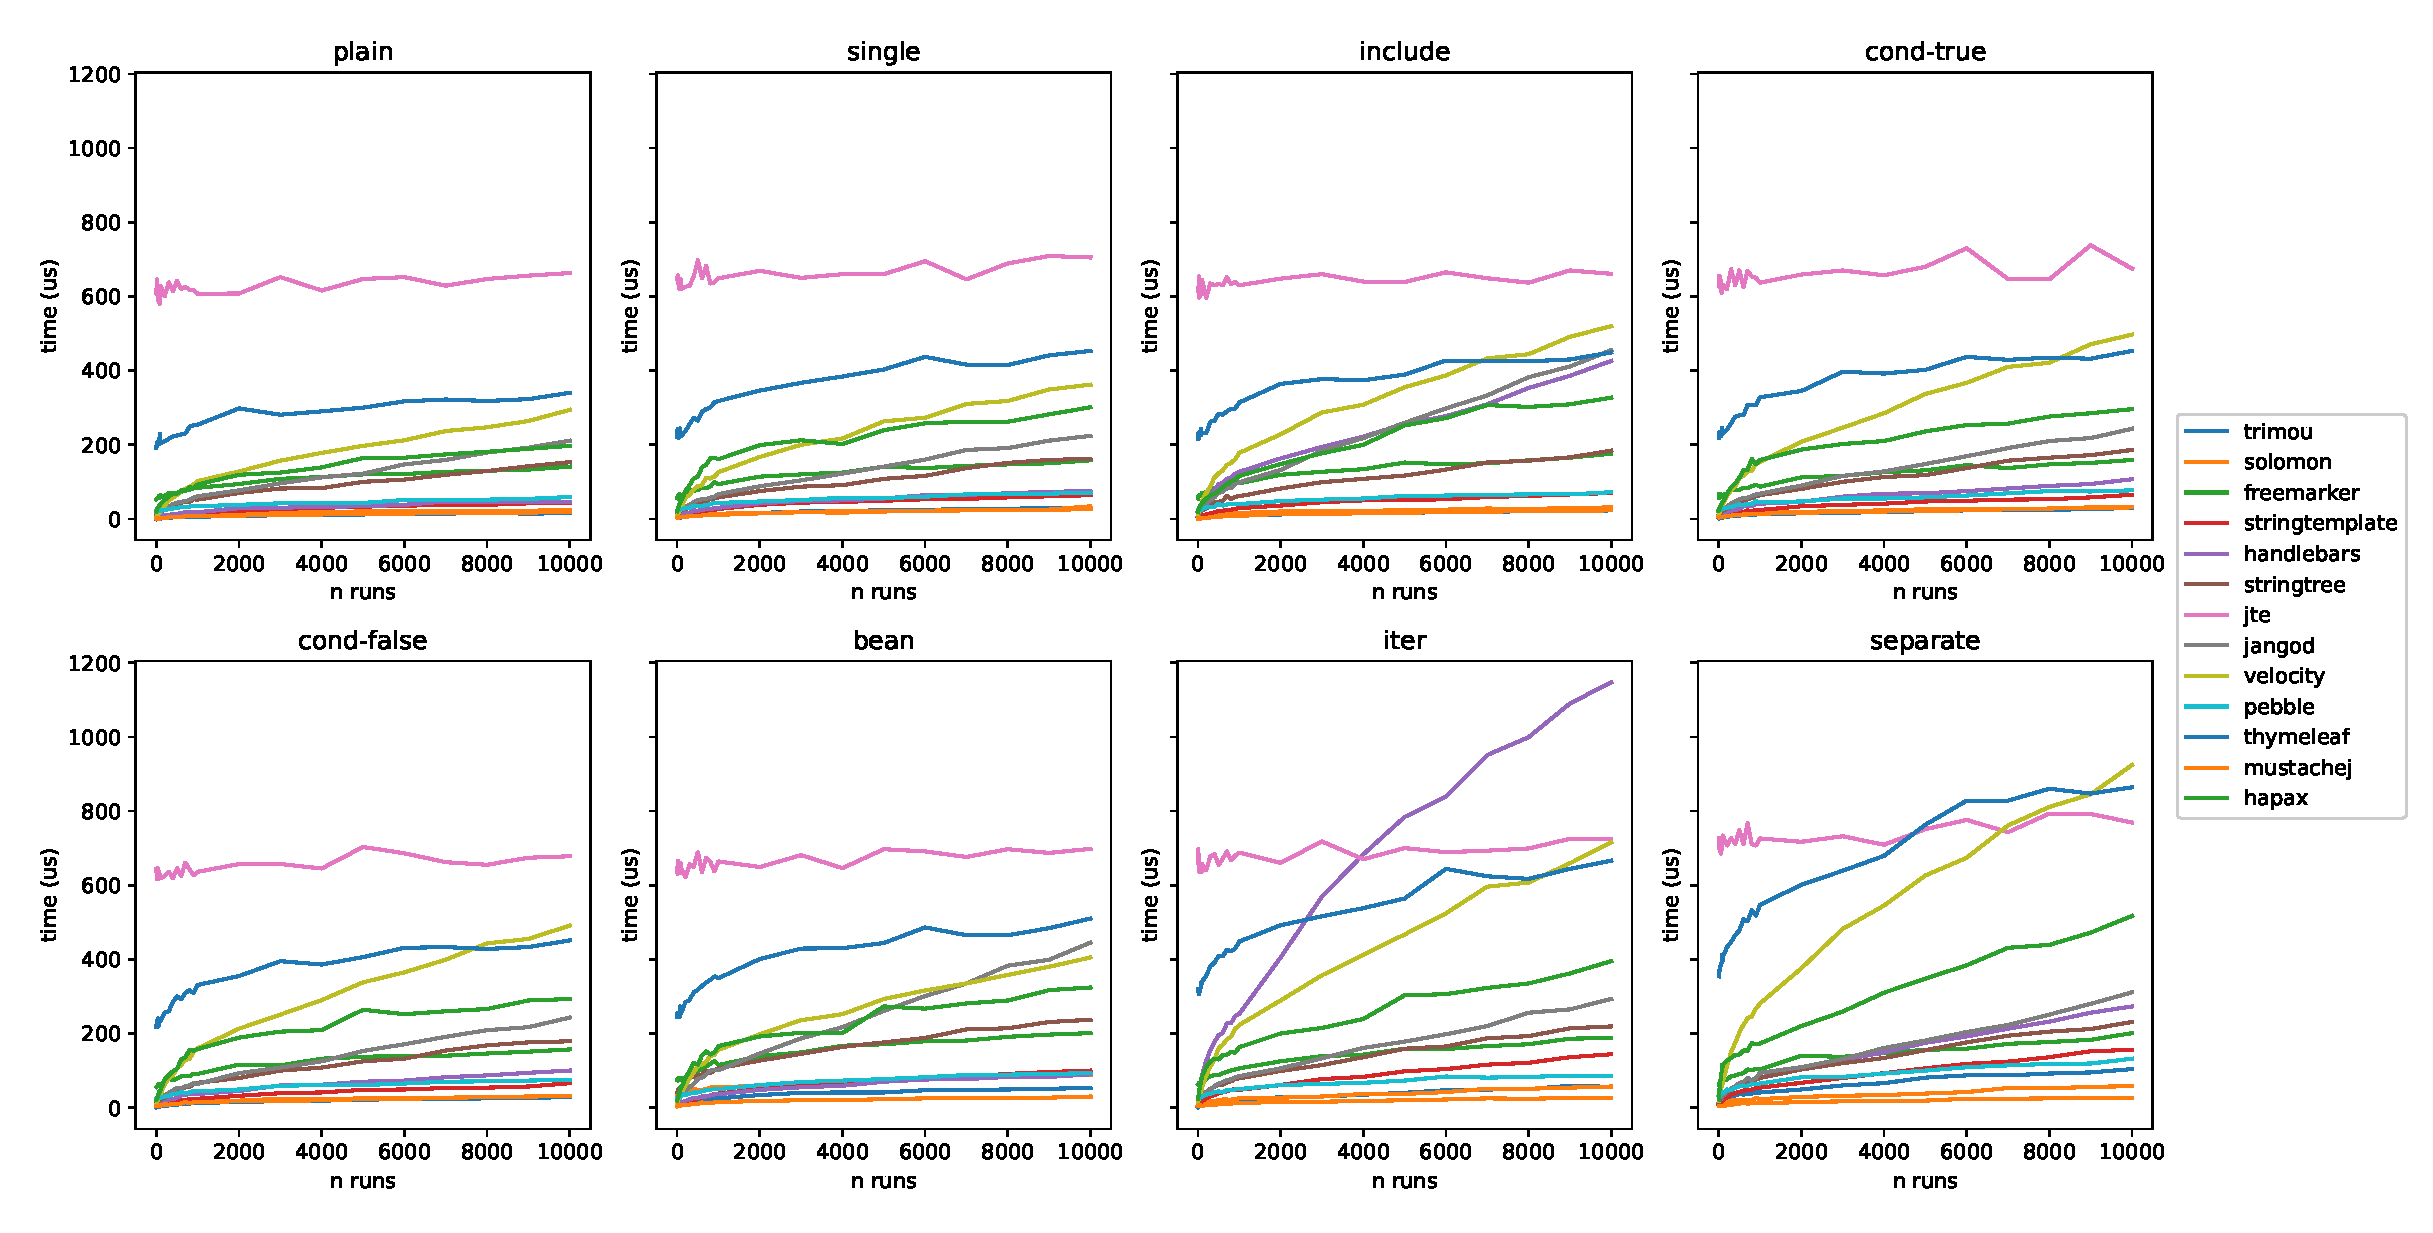
\includegraphics[width=\columnwidth]{Figures/graphs/wave4/2023-12-19-avg.eps}
\caption{\label{multi:wave4-average}Wave 4 Averaged over 8 Runs}
\end{figure}

Following the investigation into the poor behaviour of the \emph{Hapax} template engine in previous waves and the discovery of a profusion of messages generated during the problematic scenarios, the code for the template engine driver was modified in an attempt to remove the messages and improve performance in these cases.

The problem was relatively subtle. As described in \autoref{section:comp:plugins}, each template engine driver has two methods. One method is called to initialise the driver, and the other is called to expand a template, provided with a context and the name of the template to expand. Typically there is some form of `impedance mismatch' between the structure and data types of the provided context, and the structure and data types of the context required by each specific template engine. Most of the template engine drivers for this cohort include a short section in the \verb!expand! method to copy values from the supplied context to the required one. In the original driver for the \emph{Hapax} template engine, this section was as described in \autoref{comp:hapax:driver1}

\begin{lstlisting}[backgroundcolor=\color{black!5},escapeinside={(*}{*)},tabsize=2,label={comp:hapax:driver1},caption={Original \emph{Hapax} Context Loop},captionpos=b]
for (String key : ContextUtils.iterable(context)) {
    Object value = context.getObject(key);
    putContext(key, value);
}
\end{lstlisting}

For each context item, this code used a \verb!putContext! method which added the supplied context key and value to a \emph{Hapax}-specific context created in the \verb!init! method. This approach had been successfully used in several other template engine drivers. Most template-engine-specific context classes follow the example set by the built-in classes which implement the \verb!java.util.Map! interface. These implementations treat a `put' operation for a key which is already present in the context as an `update' operation. If the provided value is the same as the existing value, then nothing changes.

For some reason, the designers of \emph{Hapax} decided to ignore that convention and, instead, issue an warning message whenever an attempt is made to `put' a value for a key which is already present in the context. This added an overhead to every `put' of every item. In the case of \emph{Hapax}, this was also compounded by a requirement to extract items from any collections in the context and place them independently in the context with a specific naming scheme. A similar warning message was then generated for every item in every collection.

The solution to this issue was to create a new \emph{Hapax}-specific context at the start of the \verb!expand! method and discard it at the end, once template expansion is complete (see \autoref{comp:hapax:driver2}). This has its own issues, such as an accumulation of objects which need to be garbage collected, but as can be seen from the graphs in \autoref{multi:wave4.2-average}, greatly improved the performance of \emph{Hapax}, particularly in the `iter' and `separate' scenarios.

\begin{lstlisting}[backgroundcolor=\color{black!5},escapeinside={(*}{*)},tabsize=2,label={comp:hapax:driver2},caption={Updated \emph{Hapax} Context Loop},captionpos=b]
        dict = TemplateDictionary.create();
        for (String key : ContextUtils.iterable(context)) {
            Object value = context.getObject(key);
            putContext(key, value);
        }
\end{lstlisting}

As discussed in \autoref{comp:wave 3}, the \emph{Handlebars} template engine also exhibited unexpectedly slow performance in the `iter' scenario. Unlike the case for \emph{Hapax}, this did not also occur in the `separate' scenario. The difference appears to be because of a quirk in the way the Java implementation \emph{Handlebars} processes templates. Like many of the templates in this cohort, \emph{Handlebars} was designed primarily for the generation of HTML web pages. HTML is largely insensitive to whitespace. In an attempt to aid in the readability of \emph{handlebars} placeholders and directives, the template parser routinely removes excess whitespace characters within the sub-templates used for loop and conditional expressions. This allows loop and conditional directives to be laid out in a manner similar to those structures in a programming language, using newlines and indentation to indicate the contents of sub-templates.

The `iter' scenario requires each item from the collection to be separated by a single space, but every attempt to add this to the template resulted in it being removed and not included in the output. Other implementations of the \emph{handlebars} template language correctly determine that this whitespace is desired in the output, but this Java implementation appears to contain a `bug' which removes too much whitespace in this situation. In order to generate the correct output, the initial `iter' template for \emph{Handlebars} was coded using template include directive to include a file containing just a single space character. This achieved the desired output, but at the expense of greater template processing time. It appears that \emph{Handlebars} does not effectively cache included templates, and was taking extra time to process the sub-template and re-load the included template for every item in the collection.

In wave 4, an alternative approach was explored, of pre-storing a context value containing a single `space' character before expanding each template, and using that context value in a placeholder to ensure that the required space character would be included in the final output. This is not a perfect solution, as it requires an extra context value placeholder in any template which faces this problem and risks the name given for this context value clashing with the name of a context value provided by the application. This approach was, however, considerably faster than the original solution involving template inclusion, as can be seen in \autoref{multi:wave4-average}. There may be other ways to achieve this, but they had not been discovered at the time this wave of measurements were taking place.

Another problem observed during the experiments for wave 3 was the failure of the \emph{Stringtemplate} template engine to correctly include other templates. The template language used by \emph{Stringtemplate} is extensively documented and claims that such a feature is supported. Unfortunately, the code to interact with the template engine from a user application is less documented. The original design of the template engine driver for \emph{Stringtemplate} worked correctly for everything except template inclusion, so addressing the issue with template inclusion was postponed until wave 4.

The code for the original \emph{Stringtemplate} driver was written based on online examples. The \verb!expand! method looked like the code in \autoref{comp:stringtemplate:driver1}.

\begin{lstlisting}[backgroundcolor=\color{black!5},escapeinside={(*}{*)},tabsize=2,label={comp:stringtemplate:driver1},caption={Original \emph{Stringtemplate} expand method},captionpos=b]
public String expand(Context context, String templateName) {
    String template = templates.get(templateName);
    ST engine = new ST(template);
    for (String key : ContextUtils.iterable(context)) {
        Object value = context.getObject(key);
        engine.add(key, value);
    }
    return engine.render();
}
\end{lstlisting}

This seemed plausible, and worked in most cases. On further research, however, it appeared that this form of usage (create an \verb!ST! object based on a supplied template and then call its \verb!render! method) was intended as a simplified syntax for applications requiring only a single template. The created \verb!ST! object only knows about the supplied template, and has no way to locate any others, so any use of template inclusion in the supplied template will never work.

Eventually, alternative code examples and documentation were located which explained that in order to use multiple templates a \verb!StringTemplateGroup! object needed to be created and populated with templates. This code was added to the \verb!init! method of the \emph{Stringtemplate} driver, and the \verb!expand! method altered to make use of the group, as shown in \autoref{comp:stringtemplate:driver2}.

\begin{lstlisting}[backgroundcolor=\color{black!5},escapeinside={(*}{*)},tabsize=2,label={comp:stringtemplate:driver2},caption={Updated \emph{Stringtemplate} expand method},captionpos=b]
public String expand(Context context, String templateName) throws IOException {
    StringTemplate template = group.getInstanceOf(templateName);
    for (String key : ContextUtils.iterable(context)) {
        Object value = context.getObject(key);
        template.setAttribute(key, value);
    }
    return template.toString();
}
\end{lstlisting}

The results of running and averaging the wave 4 script following these changes is shown in \autoref{multi:wave4.2-average}. \emph{Handlebars} now shows a much shallower curve in the `iter' scenario, \emph{Stringtemplate} now produces the correct output for template inclusion and performs well in all the scenarios, and \emph{Hapax} remains reasonable in both the looping scenarios.

\begin{figure}[ht!]
\centering
\includesvg[width=\columnwidth]{Figures/graphs/svg/2023-12-20avg.csv.svg}
% 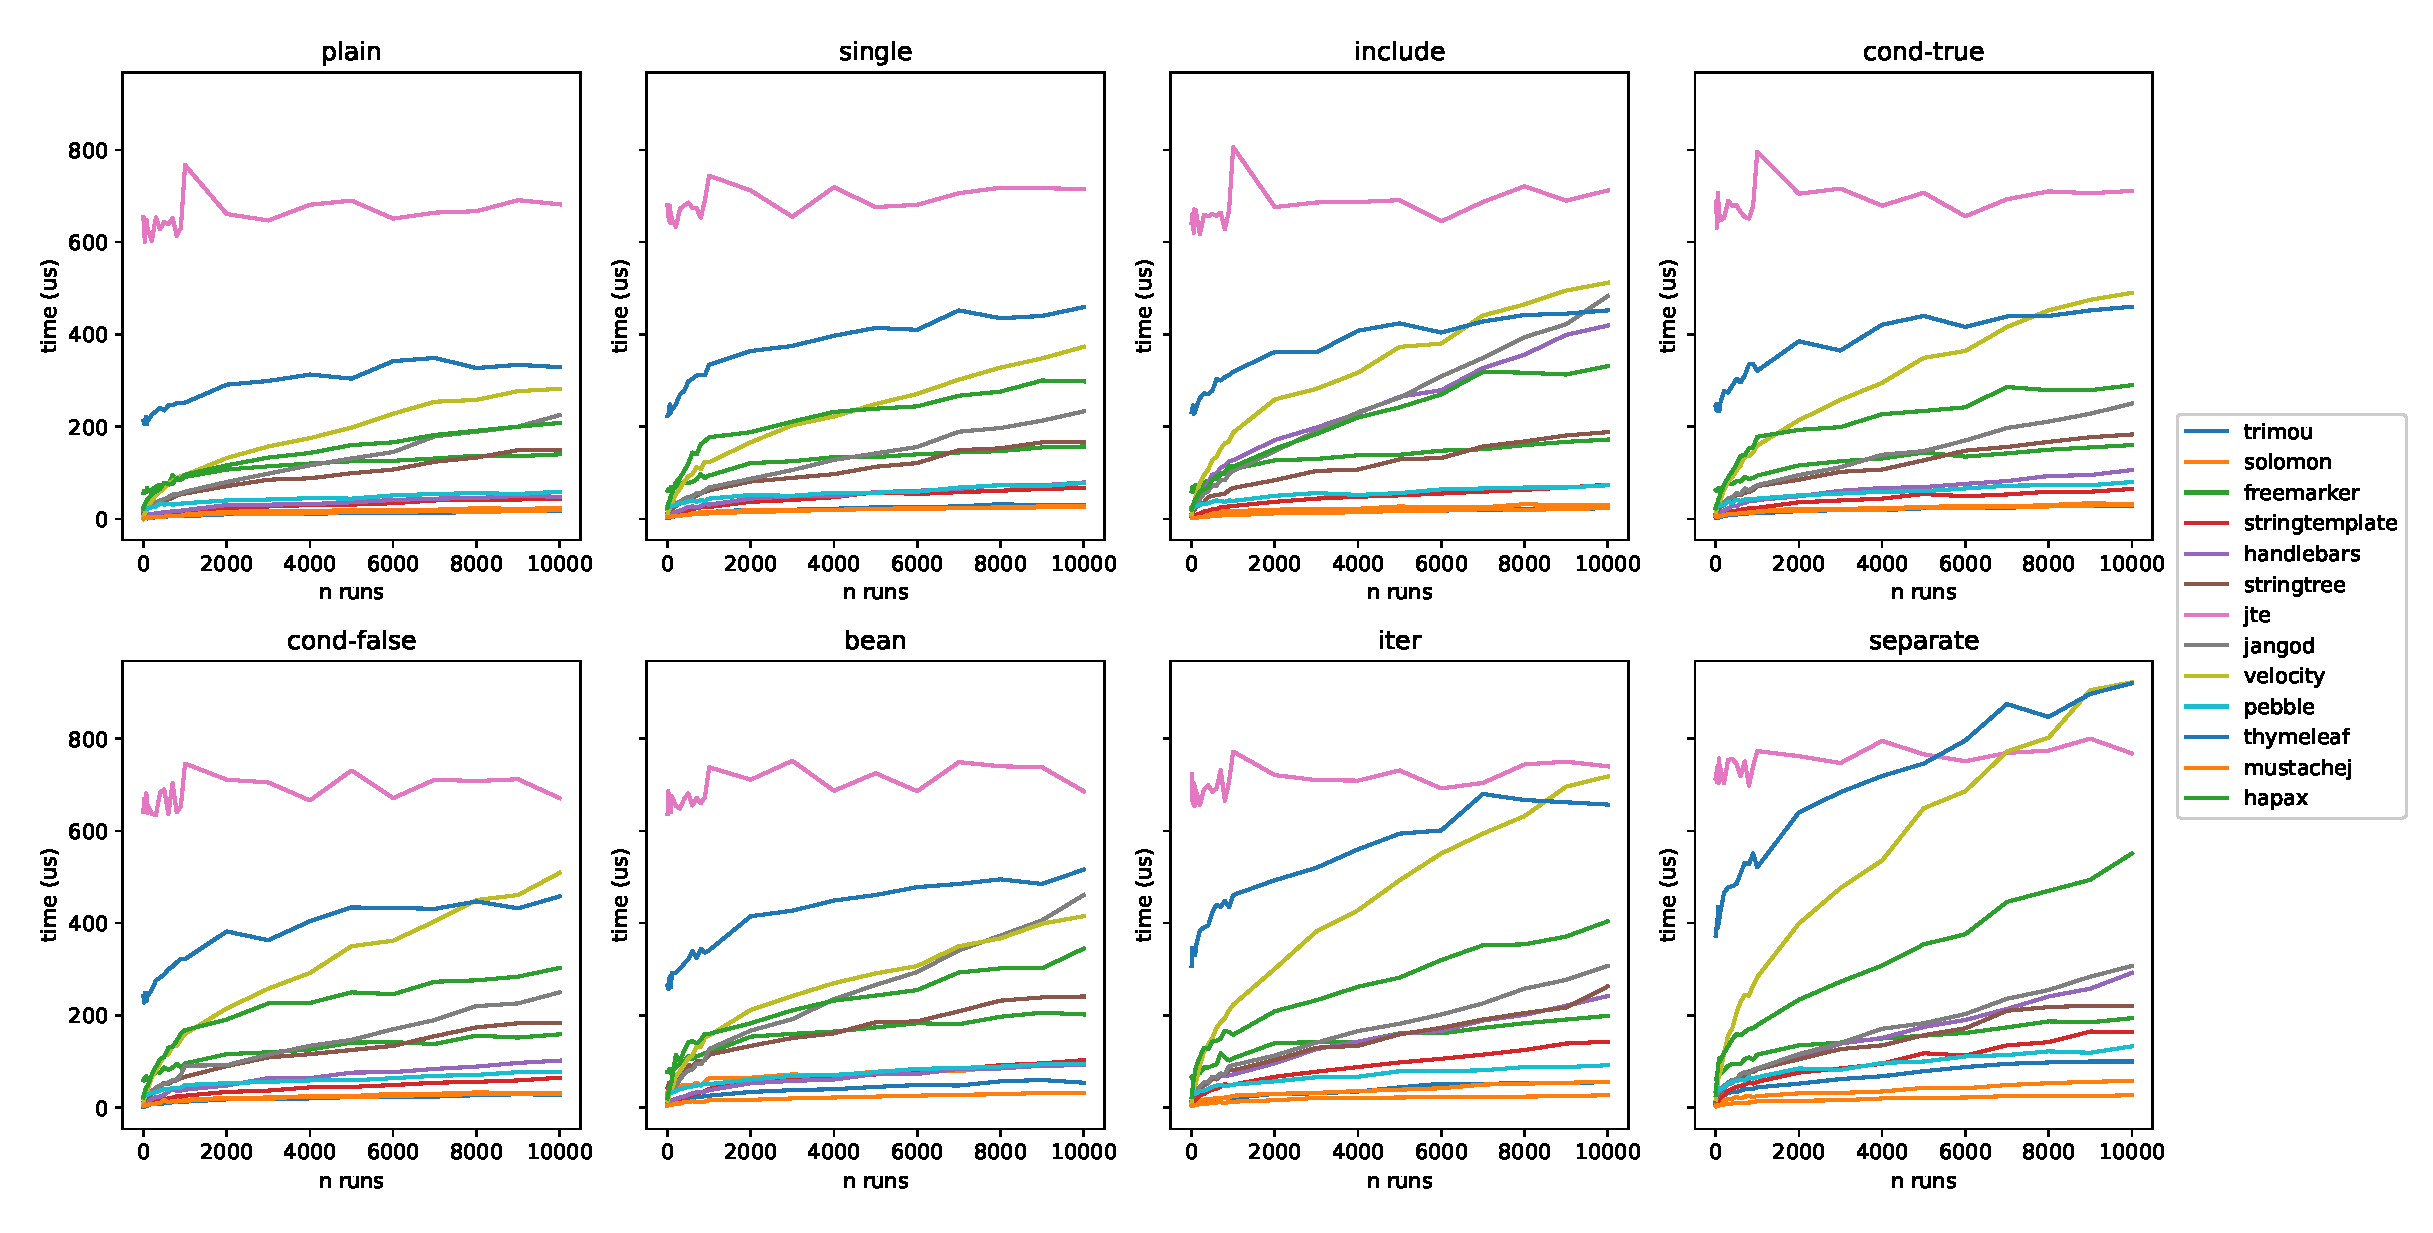
\includegraphics[width=\columnwidth]{Figures/graphs/wave4/2023-12-20avg.eps}
\caption{\label{multi:wave4.2-average}Wave 4 with updated \emph{Handlebars} and \emph{Stringtemplate}}
\end{figure}

While the graphs in \autoref{multi:wave4-average} and \autoref{multi:wave4.2-average} have eliminated some of the `noise' by averaging multiple runs, and show the general relationship between the performance characteristics of the different template engines, they are still not as smooth as the curves from wave 3 in \autoref{multi:wave3-average}. \autoref{multi:wave4.2-smooth} shows the result of applying a Savitzky-Golay filter \citep{Schafer2011} to the averaged results of the second set of wave 4 measurements.

\begin{figure}[ht!]
\centering
\includesvg[width=\columnwidth]{Figures/graphs/svg/2023-12-20-smoothed.csv.svg}
% 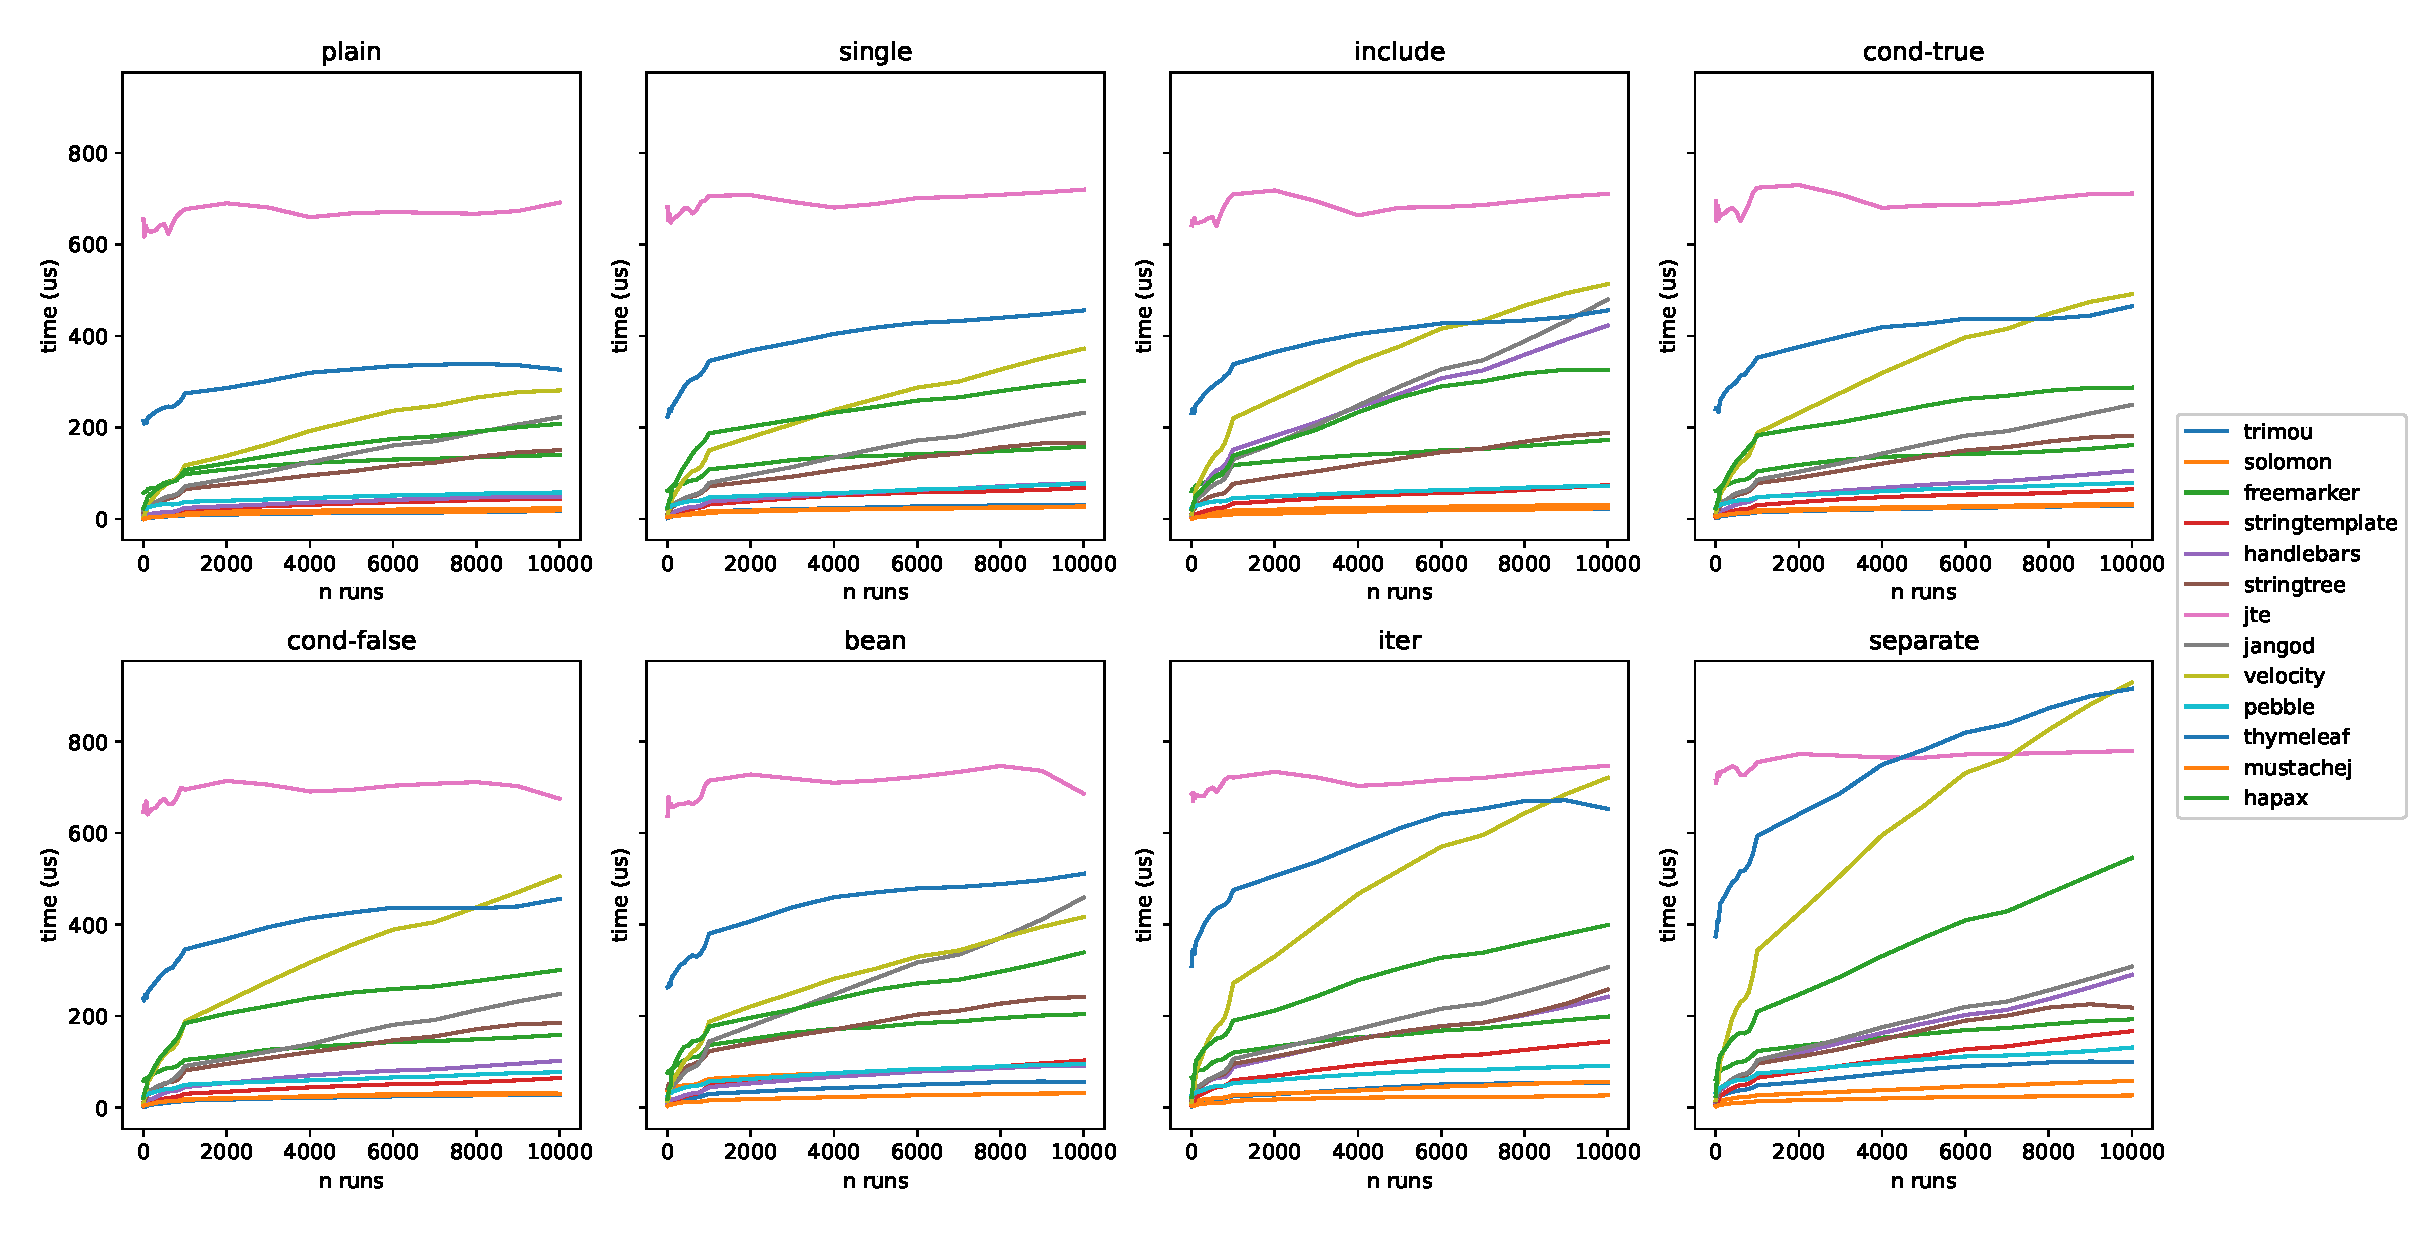
\includegraphics[width=\columnwidth]{Figures/graphs/wave4/wave4-smooth.eps}
\caption{\label{multi:wave4.2-smooth}Wave 4 with Curve Smoothing}
\end{figure}

These graphs are slightly less busy than the raw data plotted in \autoref{multi:wave4.2-average}, but also exhibit unexpected distortion of the data such as the apparent reduction in the time taken by \emph{Thymeleaf} at high numbers of template repetitions. This appears to be an artefact of the smoothing algorithm which uses a polynomial fit approach. Such smoothed graphs should therefore not be used to draw conclusions about the detail of the template engine performance.

\section{Discussion}
\label{comp:fs2:dicsussion}

The performance comparisons in this chapter exhibit a distinct difference in performance between the candidate template engines and also between the evaluation scenarios. When comparing at only a single load it can be tempting to assume that time taken scales linearly with load, but the results of these comparisons show that this does not always hold. This in turn implies that when selecting a template component based on performance, the choice should depend on the expected volume of traffic as well as other considerations.

The high minimum duration and relatively shallow slope of increase associated with the \emph{JTE} template engine may be explained by its architecture. Unlike most of the other template engines, when \emph{JTE} loads a template, it first translates it to Java code, then calls the Java compiler to compile that code to JVM \emph{bytecode} for direct execution during template expansion. This process imposes a largely constant time overhead, even when the template contains no placeholders and could be transferred directly to the output. The rest of the template engines in this cohort use a variety of approaches from re-parsing and direct interpretation of the template each time to intermediate compilation into an internal data structure on loading, followed by rendering from that data structure to reduce the overhead of re-parsing the template.

These experiments revealed several issues with the template engine components themselves. Small changes to the driver code for \emph{Hapax} made a huge difference to the performance of the component. Similarly, \emph{Handlebars} provided alternative template syntax options to achieve the same output but with large differences in performance. The performance difference between \emph{Trimou}. \emph{Mustachej} and \emph{handlebars}, which use largely similar syntax, showed that there is no direct relationship between the choice of template language syntax and the performance of the template engine.

As can be seen from the results of the individual scenario measurements in waves 1 to 4, the performance of a template engine varies depending on what is asked of it. The individual scenarios used up to this point have all been aimed at determining, and in some cases improving, the performance of each template engine for single, very specific, tasks. This is not generally how template engines are used in commercial projects, however. The most common application for template engines is the generation of web pages, and a typical web page will have multiple placeholders and directives mixed in with large blocks of boilerplate text and page markup. The creation of such templates for all the template engines in this cohort would be a complex and potentially error-prone process. An intermediate representation and a software tool to generate such templates is explored in \autoref{chapter:intermediate}. The performance of this kind of scenario is explored in more depth in \autoref{section:context energy}, which also compares the energy use of the components.

\section{Conclusions}
\label{comp:conclusions}

The most striking conclusion from this second round of template engine performance tests is the wide range of different performance profiles across the cohort of template engines tested. The initial performance tests discussed in \autoref{section:fs1} highlighted a large difference in performance for one particular number of repetitions, but further investigation clearly shows that this relationship is not true for all scenarios and workloads. Some template engines have a large initial performance cost, but relatively stable performance regardless of the number of repetitions. Others show execution times which increase with the number of repetitions, but at a wide range of slopes. The relationship between duration and workload is also not the same for the different template scenarios. Some scenarios, such as ones involving iteration, appear to cause some template engines to work much harder and therefore take longer. The initial configuration of \emph{Hapax}, for example, took so long to process the iteration scenarios that the results for other template engines were barely visible.

From a sustainability perspective, it is not enough just to measure and compare performance. There must also be some usable outcome. The usable outcomes which arose from the measurements during the several waves of this investigation into template engine performance were twofold.

\begin{itemize}
    \item The first outcome was a better understanding of the characteristics of the performance of each of the template engines, which in turn led to an understanding that template engine performance can vary considerably by both scenario and volume. Both of these criteria need to be considered when selecting candidate components.
    \item The second outcome was a recognition of the scale of the difference made by seemingly small changes in the way a template engine is used or how templates are constructed. Selecting a template engine without understanding of these areas could result in software which generates correct output documents, but risks very poor performance. 
\end{itemize}

Such poor performance might in turn result in the software system either not achieving its goals or requiring considerably more computing resources, with the accompanying consumption of materials and energy, and emission of greenhouse gasses, to achieve them.

Understanding software component performance characteristics, then using that understanding to select appropriate components and configure and use them correctly could therefore be a direct contribution to increasing the sustainability of software systems.
